\documentclass[10pt, a4paper]{article}

\usepackage[a4paper, top=0.5cm, bottom=0.5cm, left=0.5cm, right=0.5cm, landscape]{geometry}
\usepackage{mathtools}
\usepackage{amsfonts}
\usepackage{multicol}
\usepackage{setspace}
\usepackage{graphicx}


\author{Zachary Chua Yan Ern}
\date{16 September 2020}
\setstretch{1.25}

\begin{document}
	\scriptsize %tiny
	\setlength\parindent{0pt}
	\setlength{\columnseprule}{0.1pt}
	
	\begin{center}
		{\large CS2100 CheatSheet}\\
		by Zachary Chua
	\end{center}
	
	\begin{multicols*}{3}
		
		{\normalsize\textbf{C programming}}\\
		\textbf{Variables}\\
		Contains name, data type, address and value (modifiable)\\
		Declaration and initialisation: \texttt{int count = 3}\\
		Without initialisation, vairable contains unknown value, not 0\\
		
		\textbf{Data Types}\\
		1. int (integer): 4 bytes, -2,147,483,648 $(-2^{31})$ to 2,147,483,647 $(2^{31} - 1)$\\
		2. float (real number): 4 bytes\\
		3. double (real number): 8 bytes\\
		4. char (character): 1 byte, enclosed in pair of single quotes eg. 'a'\\
		
		\textbf{Preprocessor Directives}\\
		1. Include libraries eg. \texttt{\#include <math.h>}, need to compile with \texttt{-lm} if imported math lib\\
		2. Macro expansions eg. \texttt{\#define PI 3.142 //use CAPS for macro}
		Macro expansions do a textual substitution\\
		
		\textbf{Input/Output}\\
		Input/Output statements:\\
		- scanf( format string, input list );\\
		- printf( format string );\\
		- printf( format string, print list )\\
		Format Specifiers\\
		
		\begin{tabular}{ | c | c | c |}
			\hline
			Placeholder & Variable Type & Function Use \\
			\hline
			\%c & char & printf / scanf\\
			\hline
			\%d & int & printf / scanf\\
			\hline
			\%f & float or double & printf \\
			\hline
			\%f & float & printf \\
			\hline
			\%lf & double & scanf \\
			\hline
			\%e & float or double & printf (for scientific notation)\\
			\hline
		\end{tabular}\\
	
		Examples\\
		- \%5d: displays integer with width 5, right justified\\
		- \%8.3f: display real number, width of 8, 3dp, right justified\\
		
		\textbf{Operators}\\
		\textbf{Equals operator}\\
		= has the side effect of returning the value assigned\\
		
		\textbf{Arithmetic Operators and Precedence}\\
		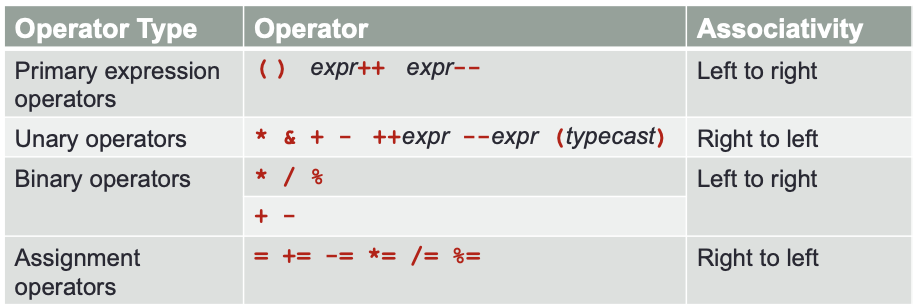
\includegraphics[scale= .5]{./assets/arithmeticOperators}\\
		Mixed-Type Arithmetic Operations\\
		- \texttt{int m = 10/4;} means \texttt{m = 2;}\\
		- \texttt{float p = 10/4;} means \texttt{p = 2.0;}\\
		- \texttt{int n = 10/4.0} means \texttt{n = 2;}\\
		- \texttt{float q = 10/4.0} means \texttt{q = 2.5;}\\
		- \texttt{r = -10/4.0;} means \texttt{r = -2;}\\
		
		\textbf{Type Casting}\\
		syntax: \texttt{ (type) expression }\\
		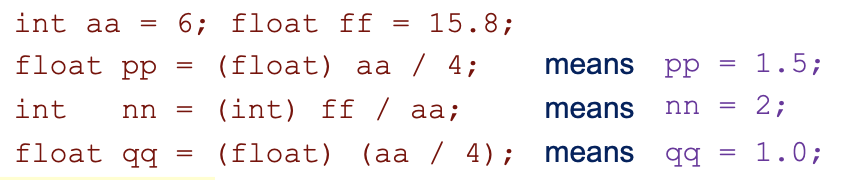
\includegraphics[scale= .5]{./assets/typeCast}\\
		
		\textbf{Remainder}\\
		\% is remainder in C\\
		- \texttt{a = 10 \% 4} $\rightarrow$ \texttt{a = 2}\\
		- \texttt{a = -10 \% 4} $\rightarrow$ \texttt{a = -2}\\
		
		\textbf{Booleans}\\
		No boolean types in C, use integers ie\\
		- 0 represents false\\
		- any other integer (usually 1) represents true\\
		
		\textbf{Operator Precedence}\\
		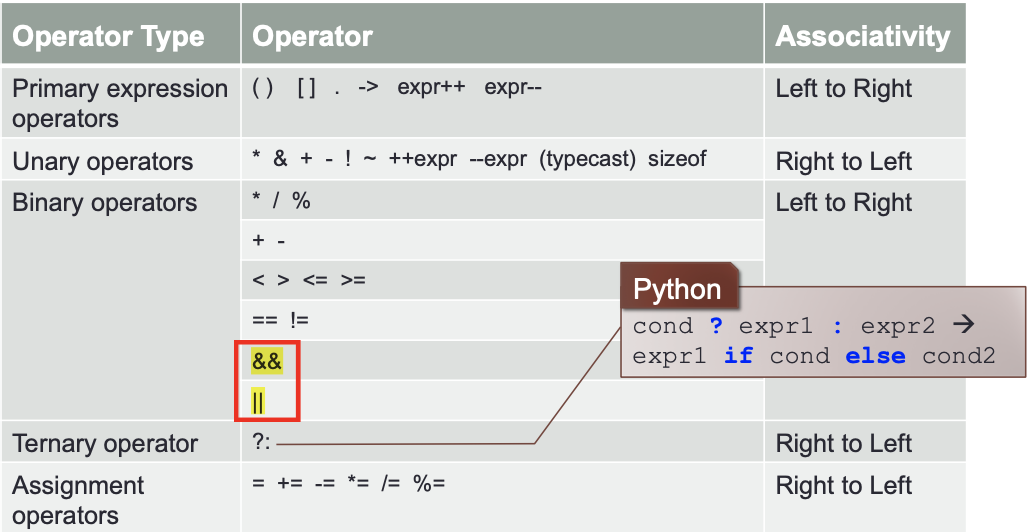
\includegraphics[scale= .5]{./assets/logicOperators}\\
		Note that precedence of $\&\&$ is greater than that of $||$\\
		$\&\&$ and $||$ use short-circuit evaluation\\
		
		\textbf{Loops}\\
		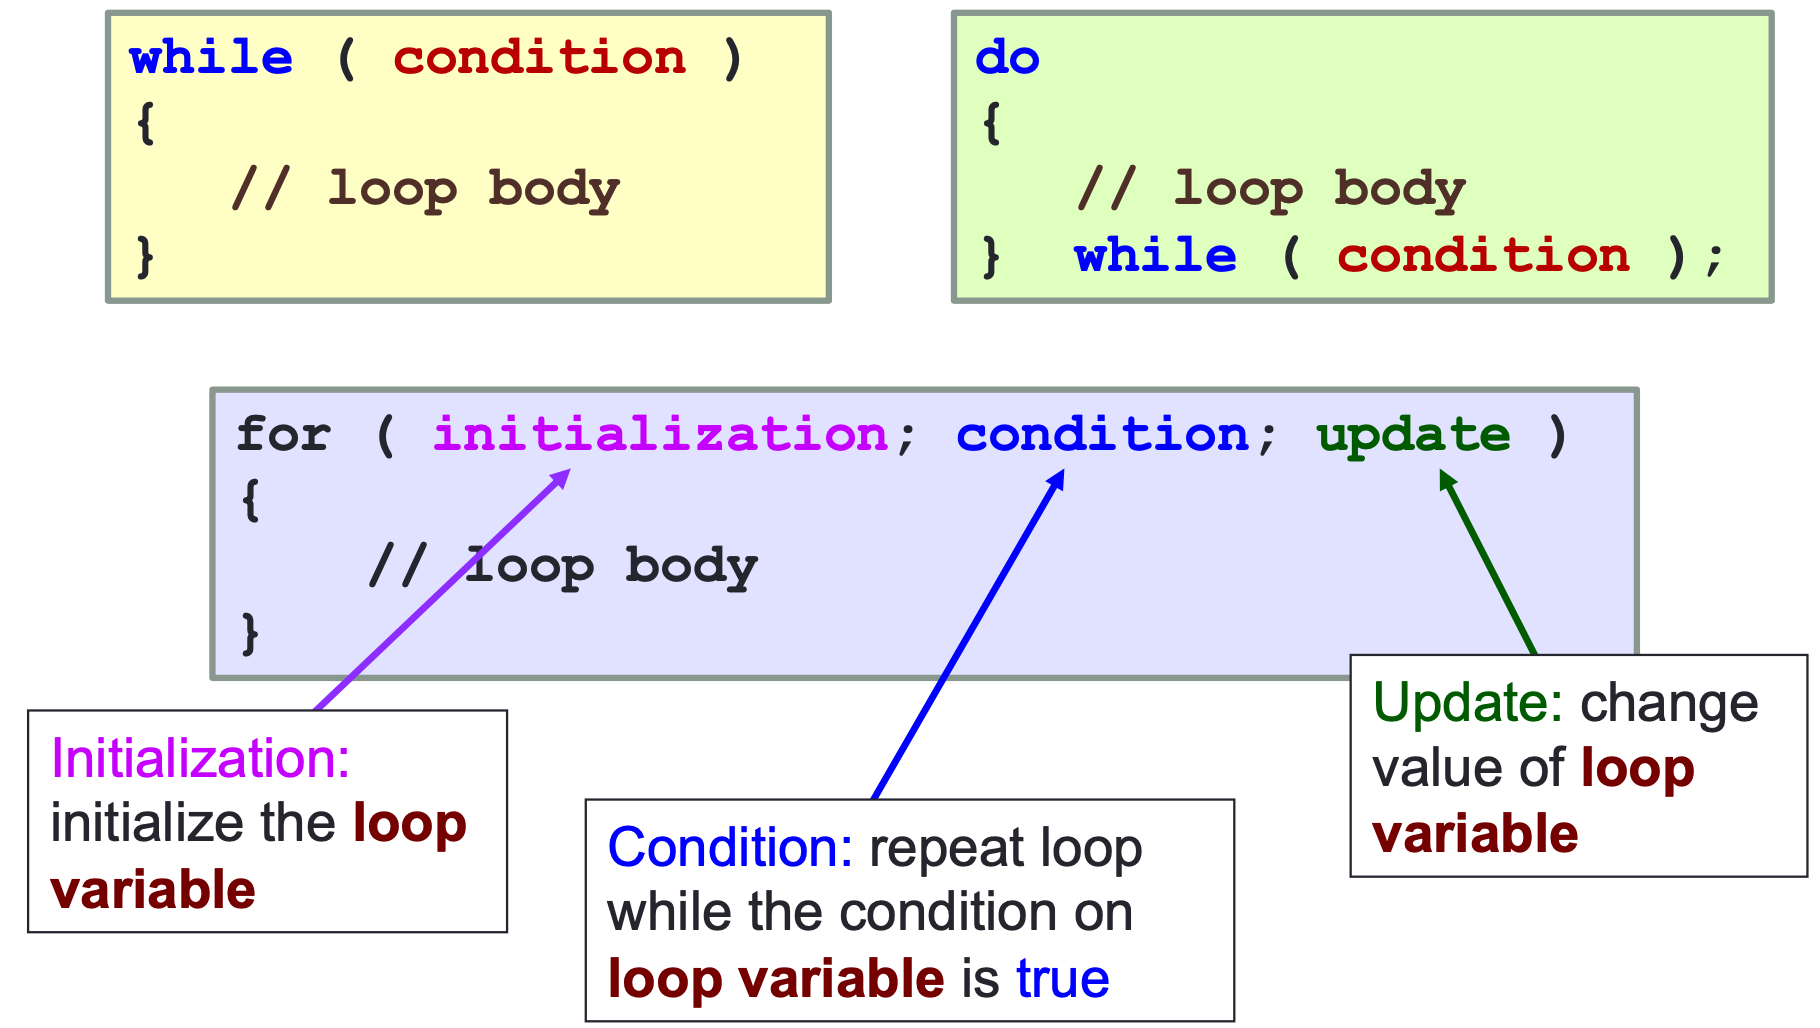
\includegraphics[scale=0.23]{./assets/loops}\\
		For \texttt{for} loops in C, declaration of the loop variable has to be before the \texttt{for} loop\\
		{\normalsize\textbf{Number Systems}}\\
		\textbf{Data Representation}\\
		- bit: 0 or 1\\
		- byte: 8 bits\\
		- word: Multiple of bytes, 4 for mips32\\
		$N$ bits can represent up to $2^N$ values, from $0 - (2^N - 1)$\\ 
		To represent $M$ values, $\lceil{log_2^M}\rceil$ bits are required\\
		In C,\\
		- Prefix 0 for octal, eg $032$ represents $(32)_8$\\
		- Prefix 0x for hexadecimal, eg $0x32$ represents $(32)_16$\\
		
		\textbf{Convertion from Decimal to Base $R$}\\
		- Whole numbers: repeated division by R until quotient 0\\
		eg for decimal to binary\\
		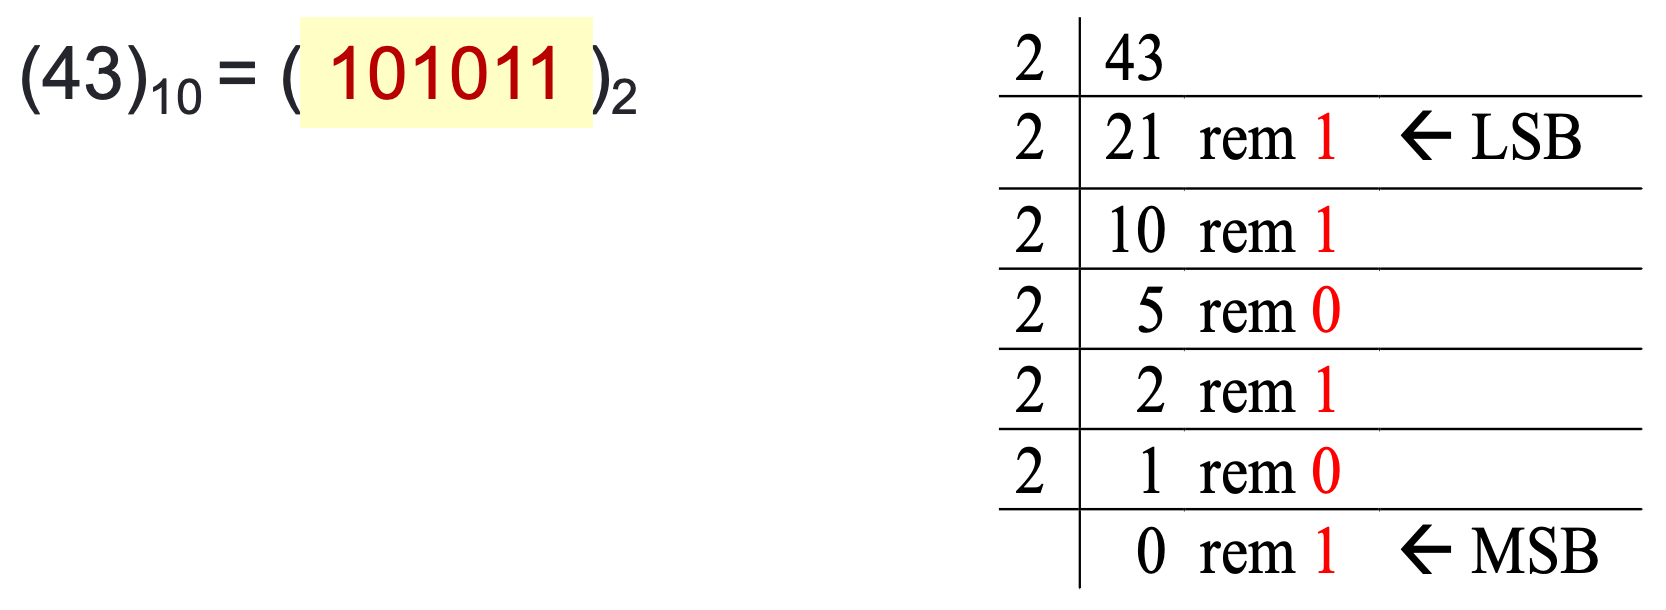
\includegraphics[scale=0.25]{./assets/baseConversion}\\
		- Fractions: repeated multiplication by R until fractional product is 0, taking the carry\\
		eg decimal to binary \\
		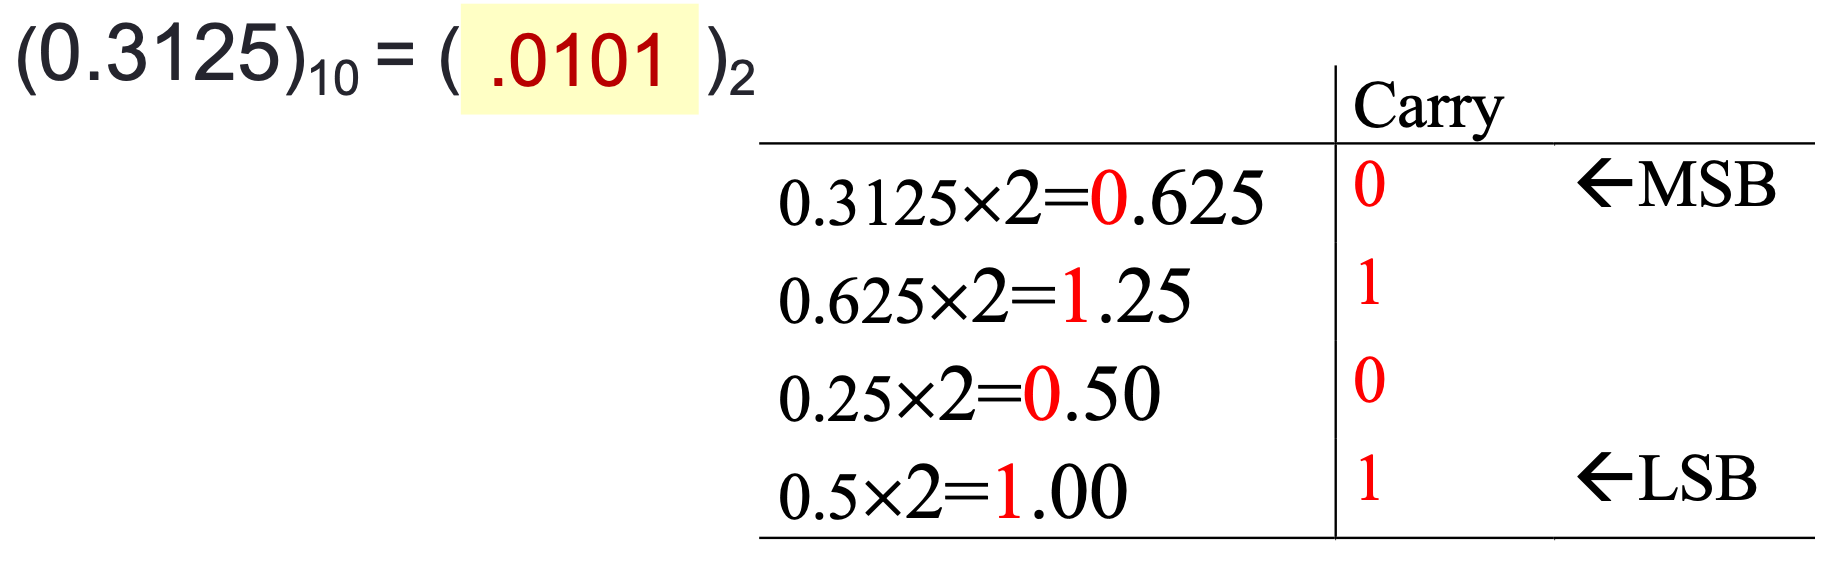
\includegraphics[scale=0.25]{./assets/baseConversion2}\\
		
		\textbf{Binary to Octal and Hexa shortcuts}\\
		- Binary to Octal: partition in groups of 3, take the value of the groups\\
		- Octal to Binary: reverse
		- Binary to Hexa: partition in groups of 4, take the value of the groups\\
		- Hexa to Binary: reverse, convert hexa to binary, extend to 4 digits if needed\\
		
		\textbf{ASCII code}\\
		Integers $(0 - 127)$ and characters are 'somewhat' interchangeable in C\\
		
		\textbf{Negative Numbers}\\
		3 representations\\
		1. Sign-and-Magnitude\\
		2. 1s complement\\
		3. 2s complement\\
		
		\textbf{Sign and Magnitude}\\
		Sign is represented by sign bit; 0 for $+$ and 1 for $-$\\
		First bit is sign bit, other 7 bits are read as normal\\
		- Largest value: $2^{n - 1} - 1$\\
		- Smallest value: $-2^{n - 1} + 1$\\		
		- 2 zeroes: $+0 = 00000000$ and $-0 = 10000000$\\
		- Range: $2^{n - 1} - 1$ to $-2^{n - 1} + 1$\\
		To negate the number, just invert sign bit\\
		
		\textbf{1s Complement}\\
		Negated value of $x$ is given by $-x = 2^n - x - 1$\\
		- Largest value: $2^{n - 1} - 1$\\
		- Smallest value" $- 2^{n - 1} - 1$\\
		- 2 Zeroes: $+0 = 00000000$ and $-0 = 11111111$\\
		- Range: $-(2^{n - 1} - 1)$ to $2^{n - 1} - 1$\\
		To negate a number, invert all bits\\
		Note that the first bit still represents the sign: 0 for positive and 1 for negative.\\
		
		\textbf{2s Complement}\\
		Negated value of $x$ is given by $-x = 2^n - x$\\
		- Largest value: $2^{n - 1} - 1$\\
		- Smallest value: $-2^{n - 1}$\\
		- Range: $-2^{n - 1}$ to $2^{n - 1} - 1$\\
		To negate a number, invert all bits, then add 1\\
		For fractions same thing, flip then add one to LSB\\
		Note that MSB still represents the sign, and that MSB "has a value" of $-2^{n - 1}$\\
		
		\textbf{Sign Extension}\\
		For 1s and 2s complement: Extend sign bit\\
		For SaM: Pad 0s after the sign bit\\
		
		\textbf{Arithmetics}\\
		\textbf{2s Complement Addition and Subtraction}\\
		Algorithm for adding integers $A$ and $B$\\
		1. Perform binary addition on the two numbers\\
		2. Ignore the carry out of MSB\\
		3. Check for overflow, overflow occurs if the 'carry in' and 'carry out' of the MSB are different. Or if the result is opposite sign of $A$ and $B$\\
		
		Algorithm for Subtraction of $A$ and $B$, $A - B = A + (-B)$\\
		1. Take 2s complement of B\\
		2. Add 2s complement of B to A, using above algorithm\\
		
		\textbf{1s Complement Addition and Subtraction}\\
		Algorithm for adding integers $A$ and $B$\\
		1. Perform binary addition on the two numbers\\
		2. If there is a carry out of the MSB, add 1 to the result (at the LSB)\\
		3. Check for overflow\\
		
		Algorithm for subtraction of $A$ and $B$\\
		1. Take 1s complement of B\\
		2. Add the 1s complement of B to A\\
		
		\textbf{Overflows}\\
		Overflows are a result of addition/subtraction going beyong the range of numbers\\
		- positive add positive $\rightarrow$ negative\\
		- negative add negative $\rightarrow$ positive\\
		
		\textbf{Excess Representation}\\
		Allows the range of values to be distributed evenly between positive and negative values, using a simple translation (subtraction)
		\begin{center}
			Excess representation = Value + excess
		\end{center}
		eg for excess-8, rep = Value + 8\\
		For 4-bit  numbers, usually use excess-7 or excess-8\\
		
		\textbf{Real numbers}\\
		Numbers with fractional components\\
		
		\textbf{Fixed point representation}\\
		Number of bits allocated for whole number part and fractional part are fixed\\
		- Advantage: Easier computation\\
		- Disadvantage: smaller range for a given precision\\		
		
		\textbf{Floating point representation}\\
		IEEE 754 Floating-Point Representation\\
		3 components: sign, exponent, mantissa (fraction)\\
		Similar to standard form\\
		Radix is assumed to be 2\\
		1. Single Precision (32-bit): 1-bit sign, 8-bit exponent with excess-127, 23-bit mantissa\\
		2. Double Precision (64-bit): 1-bit sign, 11-bit exponent with excess-1023, 52-bit mantissa\\
		Mantissa normalised with an implicit leading bit 1\\
		eg. -6.5 in decimal
		\begin{center}
			$-6.5_{10} = -110.1_2 = -1.101_2 * 2^2$\\
			IEEE 754: 1 10000001 10100000000000000000000$_2$ = C0D00000$_{16}$\\
		\end{center}
		
		{\normalsize\textbf{Pointers and Functions}}\\
		\textbf{Pointers}\\
		Variables occupies some space in memory and has an address\\
		Can refer to the address of a variable by usiing the \textit{address of operator}, \&\\
		\%p is used as the format specifiier for addressses, addresses are printed out in hexadecimal format\\
		
		\textbf{Pointer Variables}\\
		Variable that contains the address of another variable.\\
		If pointer variable, a\_ptr, contains address of variable a\\
		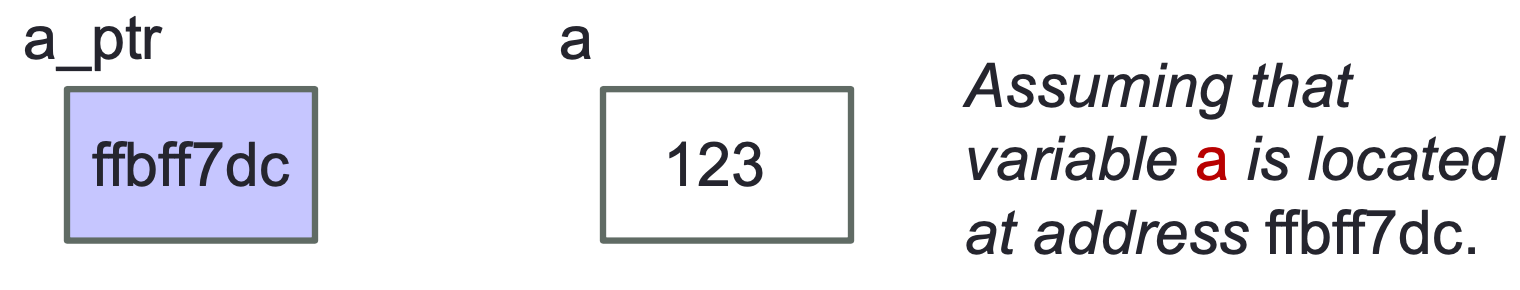
\includegraphics[scale=0.25]{./assets/pointer1}\\
		a\_ptr is said to be pointing to a\\
		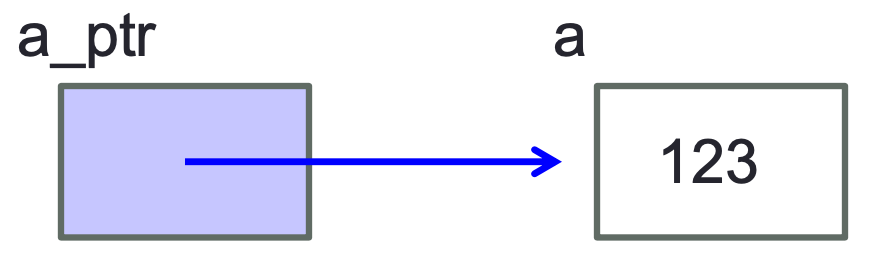
\includegraphics[scale=0.25]{./assets/pointer2}\\
		
		\textbf{Declaring a Pointer}\\
		Syntax:
		\begin{center}
			\texttt{type *pointer\_name}\\
		\end{center}
		- pointer\_name is the name of the pointer (Good practice to name a pointer with suffix \_p or \_ptr)\\
		- type is the data type of the variable this pointer may point to\\
		eg. \texttt{int *a\_ptr} declares a pointer to an int named \texttt{a\_ptr}\\
		
		\textbf{Assigning Value to a Pointer}\\
		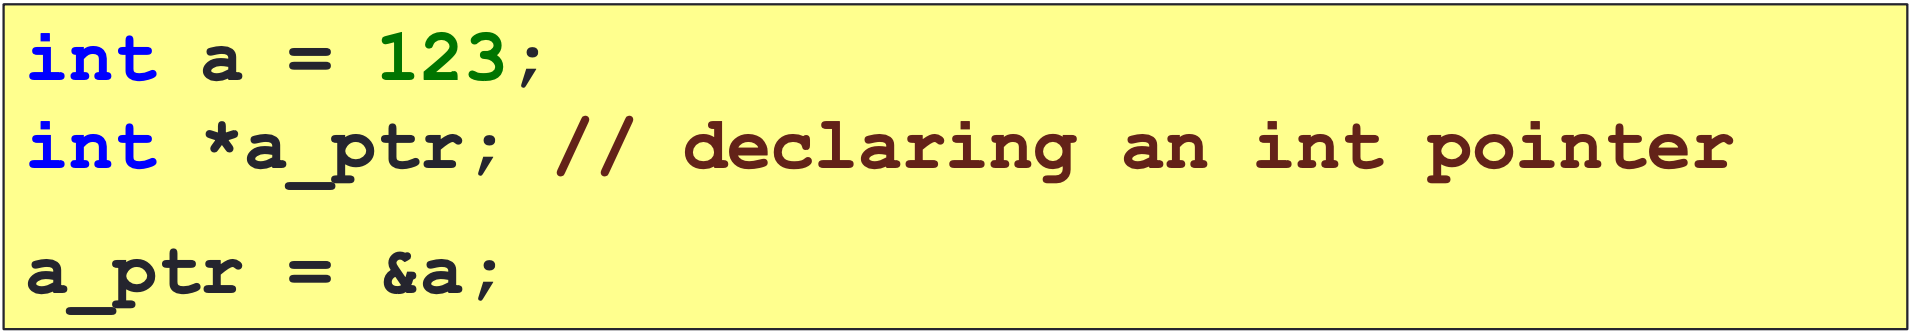
\includegraphics[scale=0.25]{./assets/pointerDeclaration}\\
		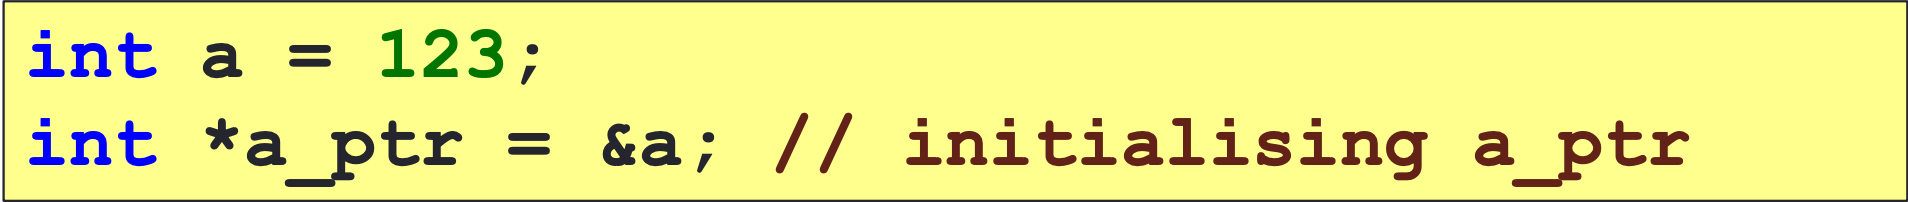
\includegraphics[scale=0.25]{./assets/pointerDeclaration2}\\
		
		\textbf{Accessing Variable through Pointer}\\
		Once a\_ptr points to a, can access a through a\_ptr using \textit{indirection operator}, (or dereferencing operator) *\\
		ie. a\_ptr* is synonymous with a\\
		
		Note that\\
		- \texttt{int *a\_ptr} is a declaration of a pointer to an int with the name a\_ptr\\
		- \texttt{*a\_ptr} is the value AT the address stored in a\_ptr\\
		
		\textbf{Incrementing Pointers}\\
		Recall that\\
		- int takes up 4 bytes\\
		- float takes up 4 bytes\\
		- char takes up 1 byte\\
		- double takes up 8 bytes\\
		Incrementing a pointer means that the pointer will look at the NEXT chunk of data,\\
		ie. incrementing an int/ float ptr increases value by 4, incrementing a char ptr increases value by 1, incrementing double ptr increases value by 8\\
		
		Note remember to assign the pointer variable an address before using if not it would be pointing somewhere unknown\\
		
		\textbf{User Defined Functions}\\
		Function Definitions follow the following syntax
		\begin{verbatim}
			return_type name(p1_type p1_name, p2_type p2_name, ...) {
				    // function body
			}
		\end{verbatim}
		Function prototypes follow the following syntax (names of params not needed)
		\begin{verbatim}
			return_type name(p1_type, p2_type, ...);
		\end{verbatim}
		Good practice to put function prototypes at the topm before main() function, after preprocessor directives. Function definitions after main() function\\
		
		Without function prototype, compiler assumes default return type of int\\
		
		\textbf{Pass-by-Value and Scope Rule}\\
		In C, actual parameters are passed to formal parameters by a mechanism called \textit{pass-by-value}\\		
		- Formal parameters and variables are local to the function they are declared in\\
		- Local parameters and variables are only accessible in the function they are declared in (Scope rule)\\
		- When function is called, activation record is created in call stack and memory is allocated for the local paramters and variables of the function\\
		- Once done, activation record is removed, memory allocated is released\\
		- Local params and variables of a function exist in memory only during execution of function and are known as \textit{automatic variables}\\
		- In contrast, \textit{static variables} live in memory even after the function is executed\\
		
		Then how to allow a function to return more than one value or modify values of variables defined outside of it?\\
		- Using functions with pointer parameters\\		
		- eg. Swap function\\
		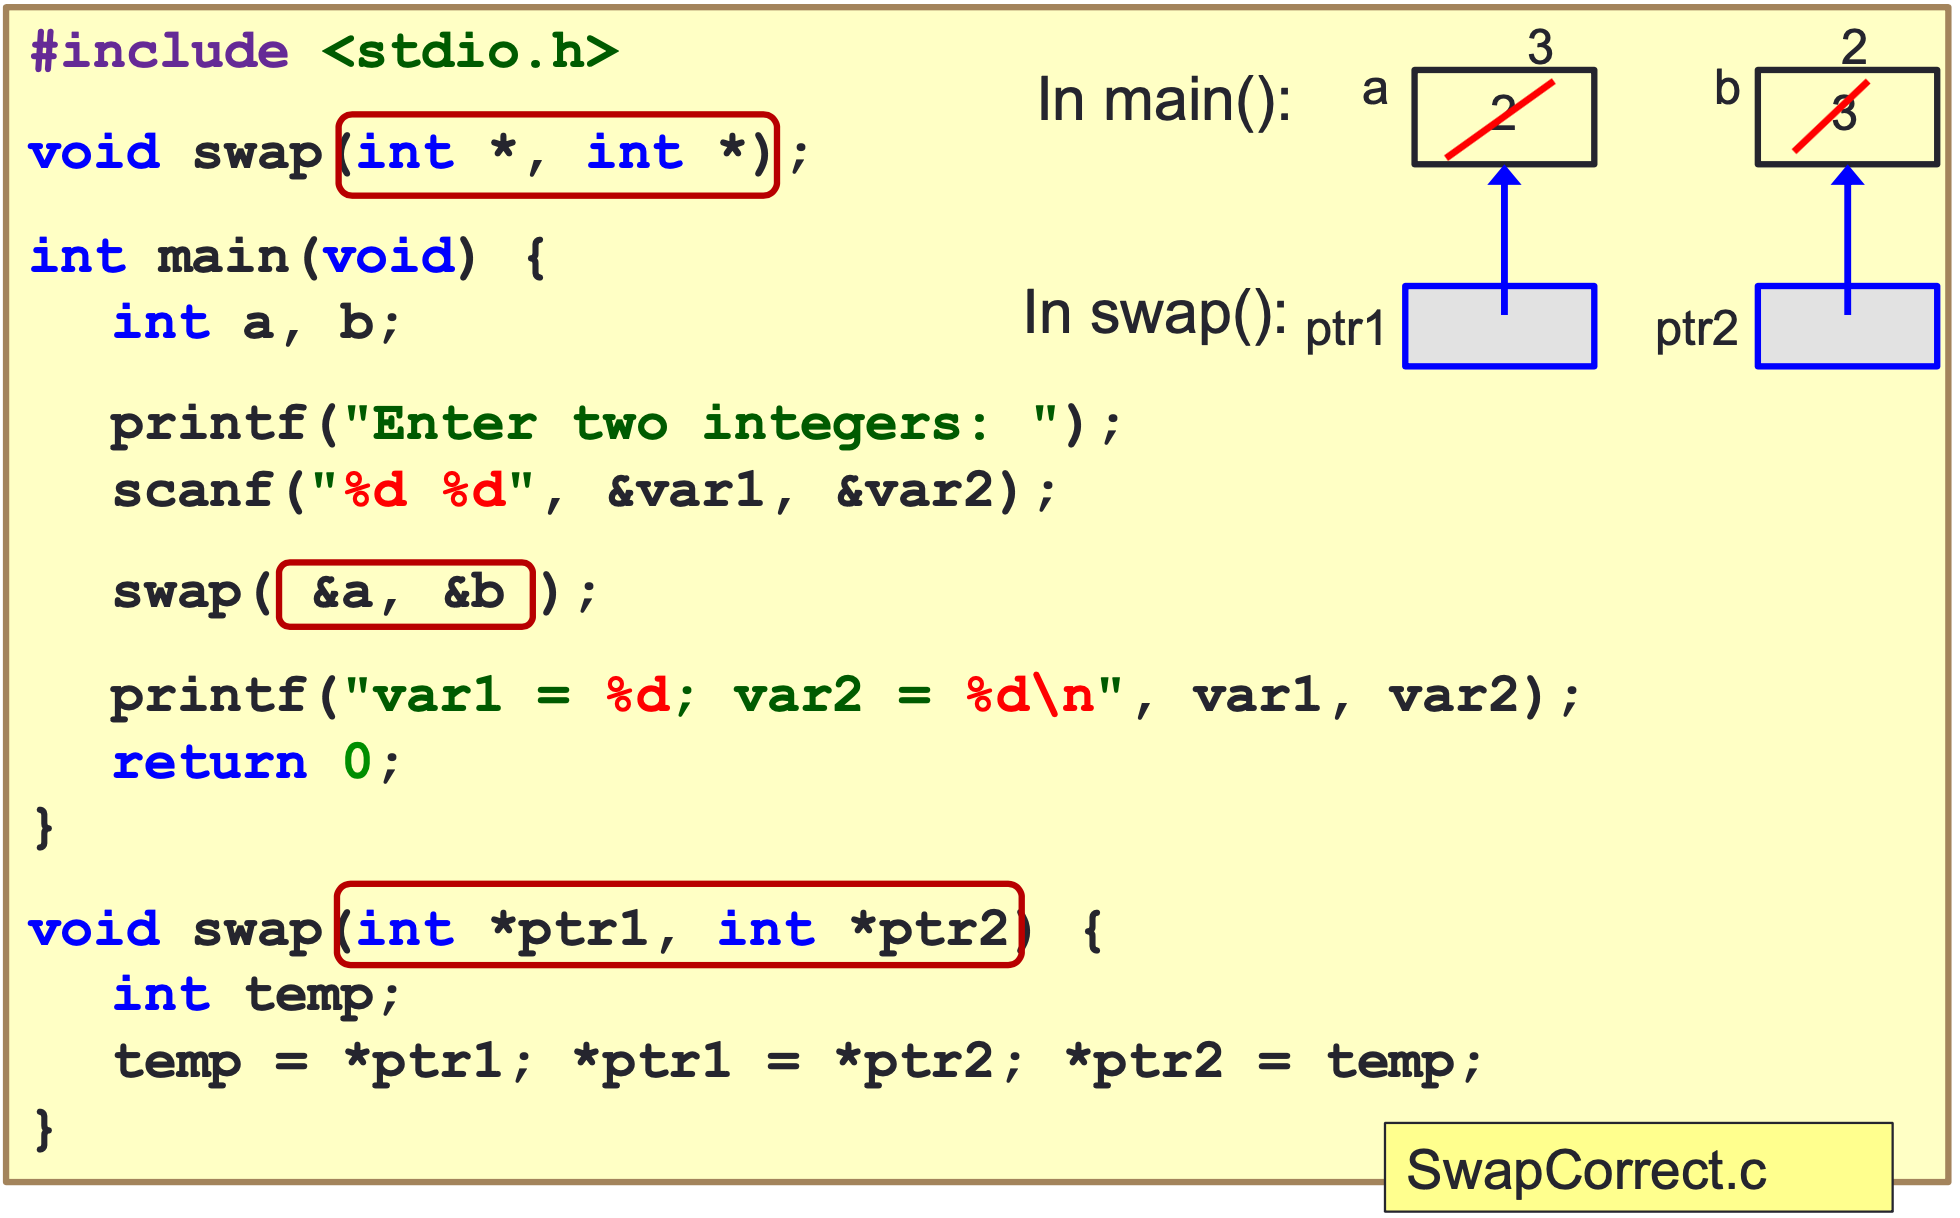
\includegraphics[scale=0.25]{./assets/swapFunction}\\
		
		{\normalsize\textbf{Arrays. Strings, Structures}}\\
		\textbf{Arrays}\\
		Declaration: element type, array name size, eg, \texttt{int c[30];}\\
		Initializing: arrays can be initialized at time of declaration\\
		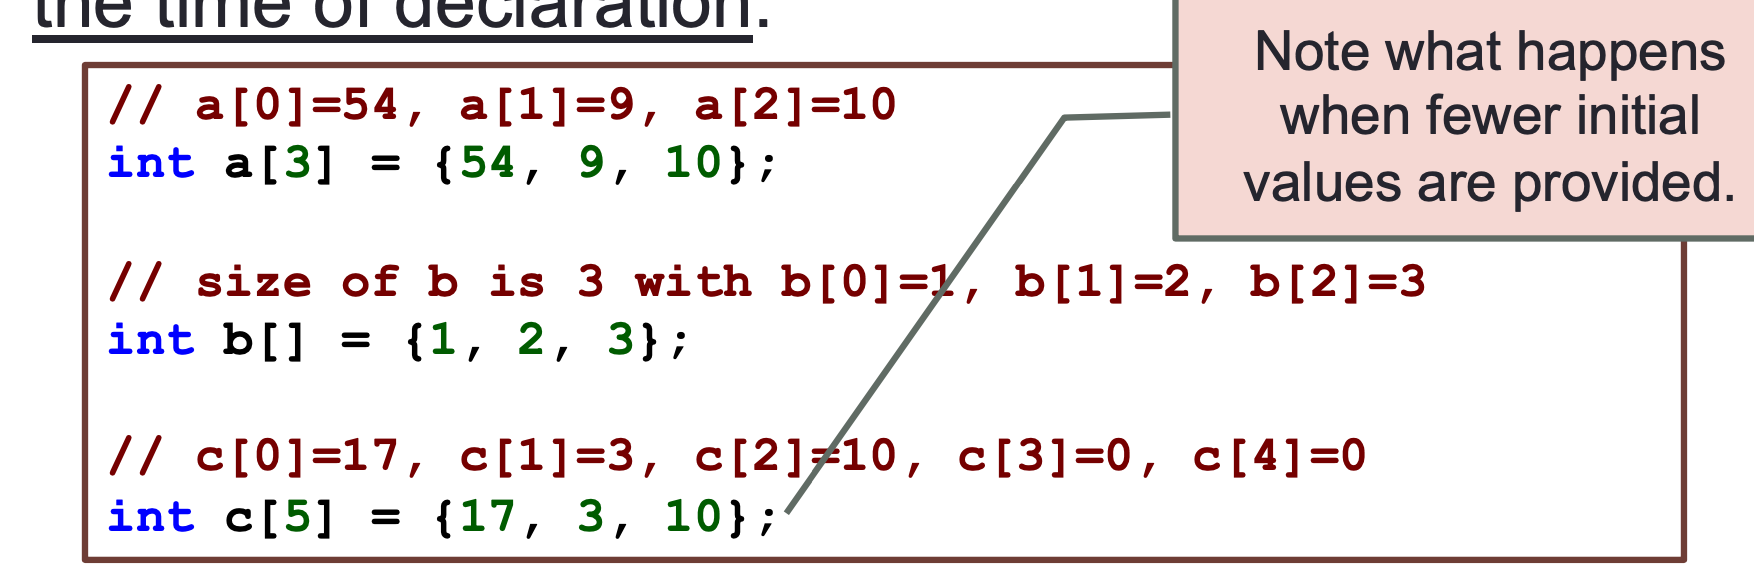
\includegraphics[scale=0.25]{./assets/array}\\
		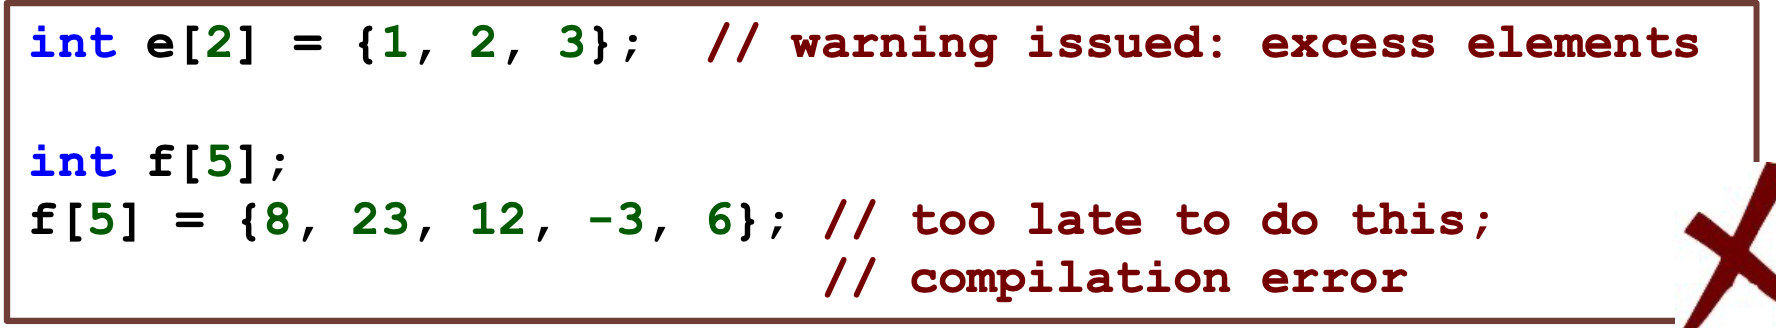
\includegraphics[scale=0.25]{./assets/array2}\\
		array name refers to the address of the first element \\
		eg. \texttt{int a[10]; // a = \&a[0]}\\
		
		\textbf{Array Assignment}\\
		Array name is a fixed pointer, it points to the first element in the array and cannot be altered
		\begin{verbatim}
			int source[10] = { 10, 20, 30, 40, 50 };
			int dest[10];
			dest = source; //illegal
		\end{verbatim}
		Instead use a loop to loop through elements and copy them over, or use \texttt{memcpy()} in $<$string.h$>$ library\\
		
		\textbf{Array params in functions}\\
		Function prototype: \texttt{int sumArray(int [], int);}\\
		Function Definition: 
		\begin{verbatim}
			int sumArray(int arr[], int size) { ... }
			int sumArray(int arr[8], int size) { ... }
		\end{verbatim}
		- Number 8 is ignored by the compiler because array parameters are passed in as pointers, must pass in size as a separate parameter\\
		- Therefore, alternative function prototype: \texttt{int sumarray(int *, size)} and alternative function definition: \texttt{ int sumArray(int *arr, int size) \{...\} }\\
		- This also means that any function can modify an array it receives\\
		
		\textbf{Strings}\\
		- Array of chars $\neq$ string, need to append null character\\
		- String is an array of chars terminated by a null character, (\textbackslash 0, ascii value 0)\\
		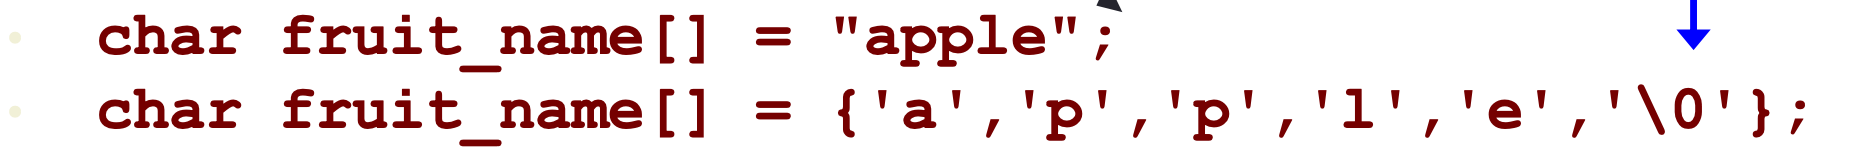
\includegraphics[scale=0.25]{./assets/stringInitialise}\\
		
		\textbf{String IO}\\
		Input:\\
		1. \texttt{fgets(str, size, stdin) // reads size - 1 char, or until (including) newline}\\
		2. \texttt{scanf("\%s", str); // reads until whitespace}\\  
		- Don't use \texttt{gets()}, can result in buffer overflow\\
		- \texttt{fgets()} can reads in newline character if there is enough space, need to replace it with null character
		\begin{verbatim}
			fgets(str, size, stdin);
			len = strlen(str);
			if (str[len - 1] == '\n') {
			    str[len - 1] = '\0';
			}
		\end{verbatim}
			
 		Output:\\
		1. \texttt{puts(str); // terminates with new line}\\
		2. \texttt{printf("\%s\textbackslash n", str); }\\
		
		\textbf{String Functions}\\
		1. \texttt{strlen(s)}, returns number of chars in s\\
		2. \texttt{strcmp(s1, s2)}, compares ASCII values of chars in s1 and s2, return negative int if s1 $<$ s2 and positive if s1 $>$ s2, 0 if same\\
		3. \texttt{strncmp(s1, s2, n)}, compares first n characters of s1 and s2\\
		4. \texttt{strcpy(s1, s2)}, copies s2 into s1, must use this because cannot assign, unless at declaration. If s2 too long can cause buffer overflow\\
		5. \texttt{strncpy(s1, s2, n)}, copies first n chars from s2 to s1\\
		All the functions use null character, without it could result in illegal access of memory\\
		
		\textbf{Structures}\\
		Structures allow grouping of heterogeneous members (of different types)\\
		A group can be a member of another group\\
		Groups are also called structure types\\
		
		Struct Definition:
		\begin{verbatim}
			typedef struct {
			    int acctNum;
			    float balance;
			} account_t;
		\end{verbatim}
		- Remember the ; at the end!\\
		- A type is NOT a variable\\
		- Types must be defined before declaring variables of that type\\
		- No memory is allocated to a type\\
		- Put struct definitions before function prototypes but after preprocessor directives\\
		
		\textbf{Accessing members of astructure variable}\\
		- Use the dot (.) operator\\
		eg:
		\begin{verbatim}
			result_t result;
			result.stuNum = 123456;
			result.score = 62.0;
			result.grade = 'D';
			
			card_t card = { 123456, {30, 6} };
			card.expiryDate.year = 2021;
		\end{verbatim}
		
		\textbf{Reading a Structure member}\\
		Structure members are read in individually
		\begin{verbatim}
			result_t result;
			printf("Enter student number, score and grade: ");
			scanf("%d %f %c", &result.stuNum, &result.score, &result.grade);
		\end{verbatim}
		Unlike arrays, can do assignment with structures, eg if result has already been initialised, result.stuNum = result1.stuNum is valid\\
		
		\textbf{Stuctures and Functions}\\
		
		Returning structure from function\\
		Can return a struct as you would for other types\\
		
		Structures as parameters\\
		- Uses pass-by-value, entire structure is copied over\\
		- To modify a structure's content, need to pass address of structure to function, using \& operator\\
		- Therefore to access members need to use (*player).name, for example. 
		- Note that dot operator (.) has higher precedence than indirection operator (*), therefore the () are needed\\
		- (*ptr\_name).member can be rewritten as ptr\_name--$>$member\\
		
		{\normalsize\textbf{MIPS}}\\
		\textbf{Overview}\\
		Mips uses Load-Store architecture, ie. both instructions and data are stored in memory\\
		- Limit memory operations\\
		- Rely on registers (mips has 32) for storage during execution\\
		Note that Registers have no data type!!\\
		Most of mips operations are register to register\\
		
		\textbf{Arithmetic Operations}\\
		Addition and Subtraction\\
		eg. texttt{add \$s0, \$s1, \$s2}, adds \$s1 and \$s2 and stores in \$s0\\
		eg. texttt{sub \$s0, \$s1, \$s2}, subtracts \$s2 from \$s1 and stores in \$s0\\		
		
		Immediate operations\\
		Immediate values are constants, 16-bit, source2 is a constant instead\\
		Values ranges from $[-2^{15}$ to $2^{15}-1]$, 16-bit 2s comp\\
		
		Register Zero\\
		\$0 always has a value of 0\\
		Can be used to assign values eg \texttt{f = g}, by writing \texttt{add \$s0, \$s1, \$zero}, f in \$s0, g in \$s1\\
		
		\textbf{Logical Operators}\\
		View Registers as 32 raw bits instead of a number\\
		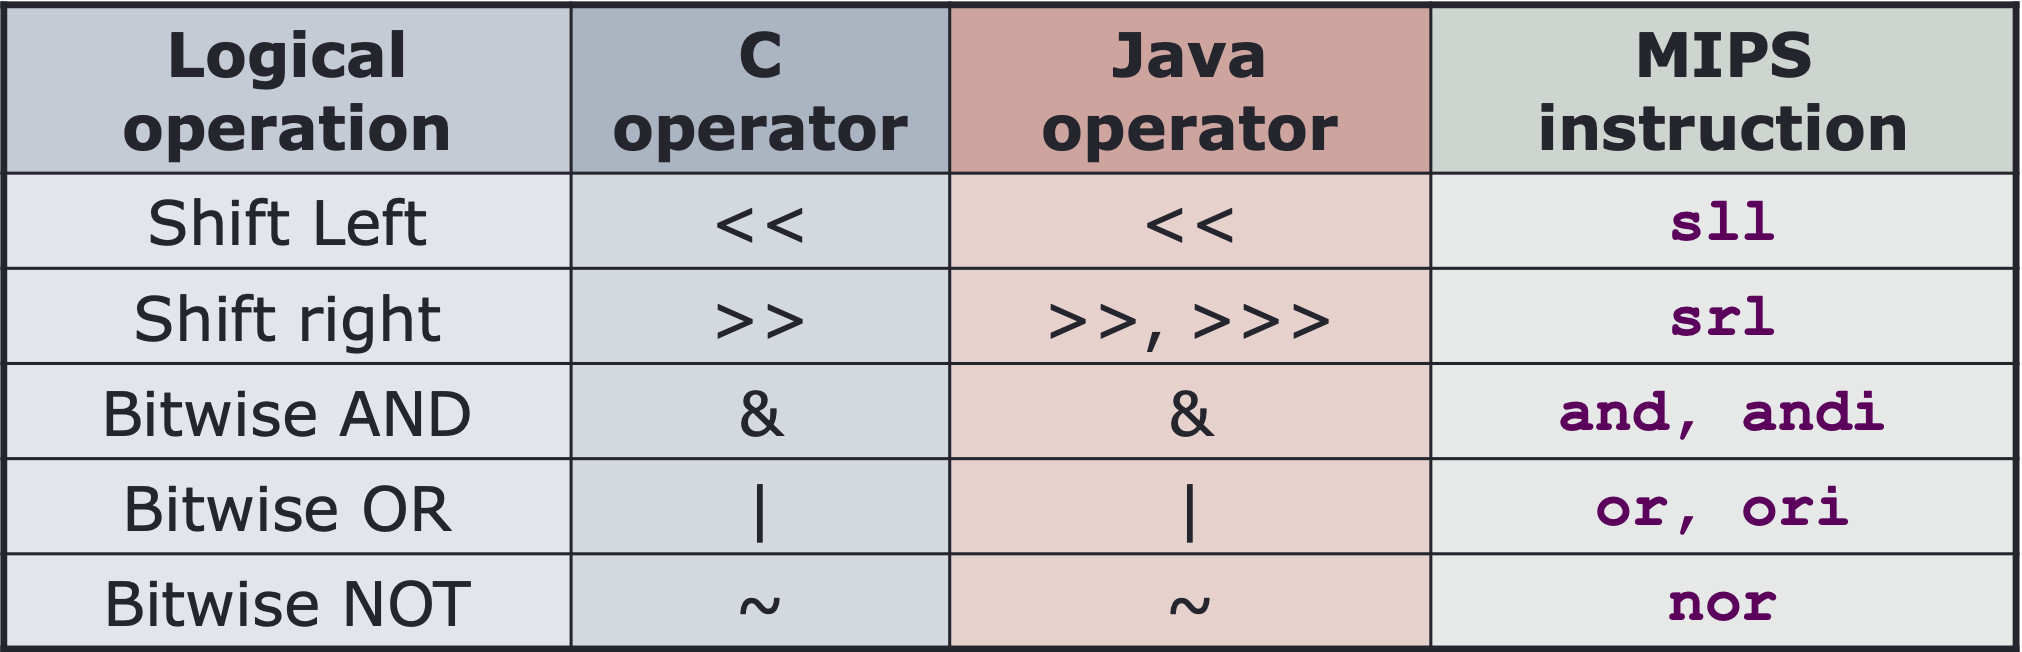
\includegraphics[scale=0.25]{./assets/logicalOperators}\\
		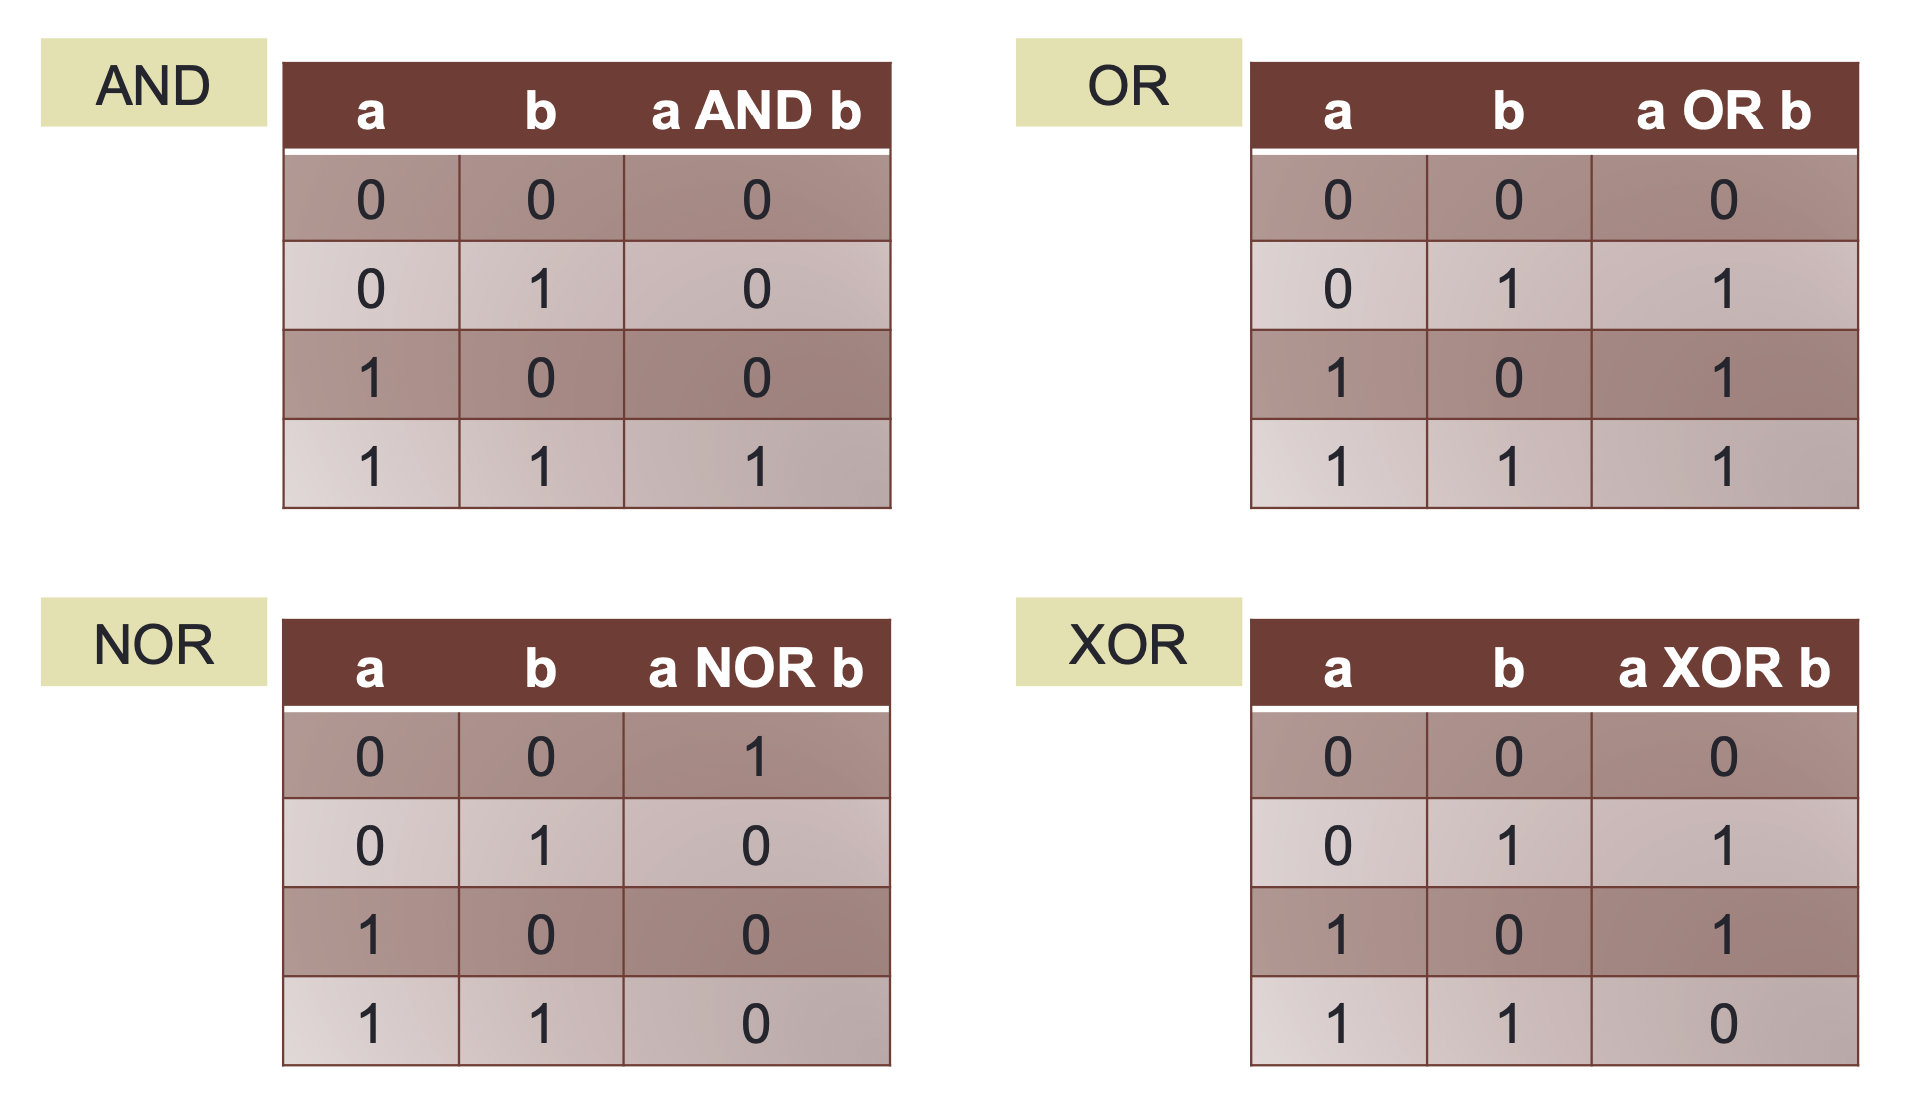
\includegraphics[scale=.25]{./assets/truthTables}\\
		
		Shift Left\\
		- sll (shift left logical): Move all bits in a word to the left by a number of positions; fill the emptied positions with zeroes.\\
		- has the effect of multiplying number by $2^n$, where n is the number in the immediate field\\
		- eg \texttt{sll \$s1 \$s1}, 3 $\rightarrow$ multiply value in s1 by 8\\
		
		Shift Right\\
		- srl (shift right logical): Move all bits in a word to the right by a number of positions; fills the emptied positions with zeroes.\\
		- divide number by $2^n$\\
		
		AND\\
		- $a \wedge 0 \implies 0$\\
		- $a \wedge 1 \implies a$\\
		- use above two properties for masking, set positions to be ignored to $0$, set positions of interest to $1$\\
		OR\\
		- $a \lor 0  \implies a$\\
		- $a \lor 1 \implies 1$\\
		- use above two properties for setting buts, set position to be set to 1\\
		
		NOR\\
		- Can be used to implement NOT instruction\\
		- NOR with 0\\		
		
		XOR\\
		- Can also be used to implement NOT instruction\\
		- XOR with 1\\
		- Has XORI instruction but no NORI, to keep instruction set small\\
		
		Large constant\\
		- How to load a 32 bit constant into a register? Recall instructions only have 16 bit immediate field\\
		- use \texttt{lui} instruction to set upper 16 bits (lower 16 bits would be set to 0)\\
		- then use \texttt{ori} instruction to set lower bits, (16 bit immediate would be 0-extended to 32-bit)\\
		Note that logical operators 0 extend immediates to 32 bits whereas arithmetic operations sign-extend(extend first bit) CHECK THIS\\
		
		\textbf{Memory Organisation}\\
		- Main memory can be viewed as a large, single-dimension array of locations.\\
		- Each location of the memory has an address (index to array), $k$ bit address $\implies 2^k$ locations\\
		- Each location/ address contains 1 byte (byte addressable), recall each word is 4 bytes long\\
		
		Word alignment\\
		- Words are aligned in memory if they begin at a byte address that is a multiple of the number of bytes in a word\\
		- Consecutive words differ by \textbf{4 bytes}\\
		
		\textbf{Memory Instruction}\\
		Load Word\\
		- eg \texttt{lw \$t0, 4(\$s0)}
		- address = value of \texttt{\$s0} + $4$, eg $8000$ stored in \texttt{\$s0}, then address = $8004$\\
		- Memory word at \texttt{Mem[8004]} loaded into \texttt{\$t0}, ie \texttt{Mem[8004] - Mem[8007]}\\
		Store Word\\
		- eg \texttt{sw \$t0, 12(\$s0)}
		- address = value of \texttt{\$s0} + $12$, eg $8000$ stored in \texttt{\$s0}, then address = $8012$\\
		- Content of \texttt{\$t0} stored into the word at \texttt{Mem[8012], ie, 8012 - 8015}\\
		
		- Note that offset for both \texttt{lw} and \texttt{sw} must be a multiple of 4 (because word is 4 bytes in mips)\\
		- MIPS does not allow unaligned load and stores with lw and sw, need to use pseudo-instructions ulw and usw\\
		- Other load-store instructions include load byte \texttt{(lb)} and store byte \texttt{(sb)}, used for chars and char arrays, for these instructions, offset no need multiple of 4\\
		
		Remember that Registers do not have type!\\
		- \texttt{lw \$t0, 0(\$s1)} then \texttt{\$s1} should contain an address\\
		- \texttt{add \$s1 \$s1 \$t0} then \texttt{\$s1} should containt a number value\\
		  
		\textbf{Decisions}\\
		Like if-else statements in higher-level languages\\
		Two types of decision-making statements in MIPS\\
		1. Conditional (branching)\\
		2. Unconditional (jump)\\
		
		\textbf{Branching}\\
		BEQ, branch on equal\\
		- eg \texttt{beq \$r1, \$r2, label}\\
		- go to the statement labeled \texttt{label} if value in \$r1 is equal to value in \$r2\\
		BNE, branch not equal\\
		- eg \texttt{bne \$r1, \$r2, label}\\
		- go to the statement labeled \texttt{label} if values aren't equal\\
		
		\textbf{Jump}\\
		- processor always follows the branch\\
		- eg \texttt{j label}\\
		
		Note that label is an "anchor" in code to indicate point of interest, usually as a branch target, Labels are not instructions\\
		- Later on labels will be converted to numbers, ie PC relative addressing for branch and truncated adress for jump\\
		Common technique: when there is only one branch, ie if with no else, then invert the conditional for more succint code\\
		
		\textbf{Inequalities}\\
		For branch on less than or branch on greater than, use slt\\
		- slt (slti): set on less than eg \texttt{slt \$t0, \$s1, \$s2}, sets \$t0 to 1 if \$s1 $<$ \$s2 or 0 otherwise\\
		- use slt with beq or bne to achieve blt or bgt (reverse \$s1 and \$s2 in slt)
		\begin{verbatim}
			blt $s1, $s2, L
			
			slt $t0, $s1, $s2 # these two instructions equivalent to above
			bne $t0, $zero, L
		\end{verbatim}
		\textbf{Arrays and loops}\\
		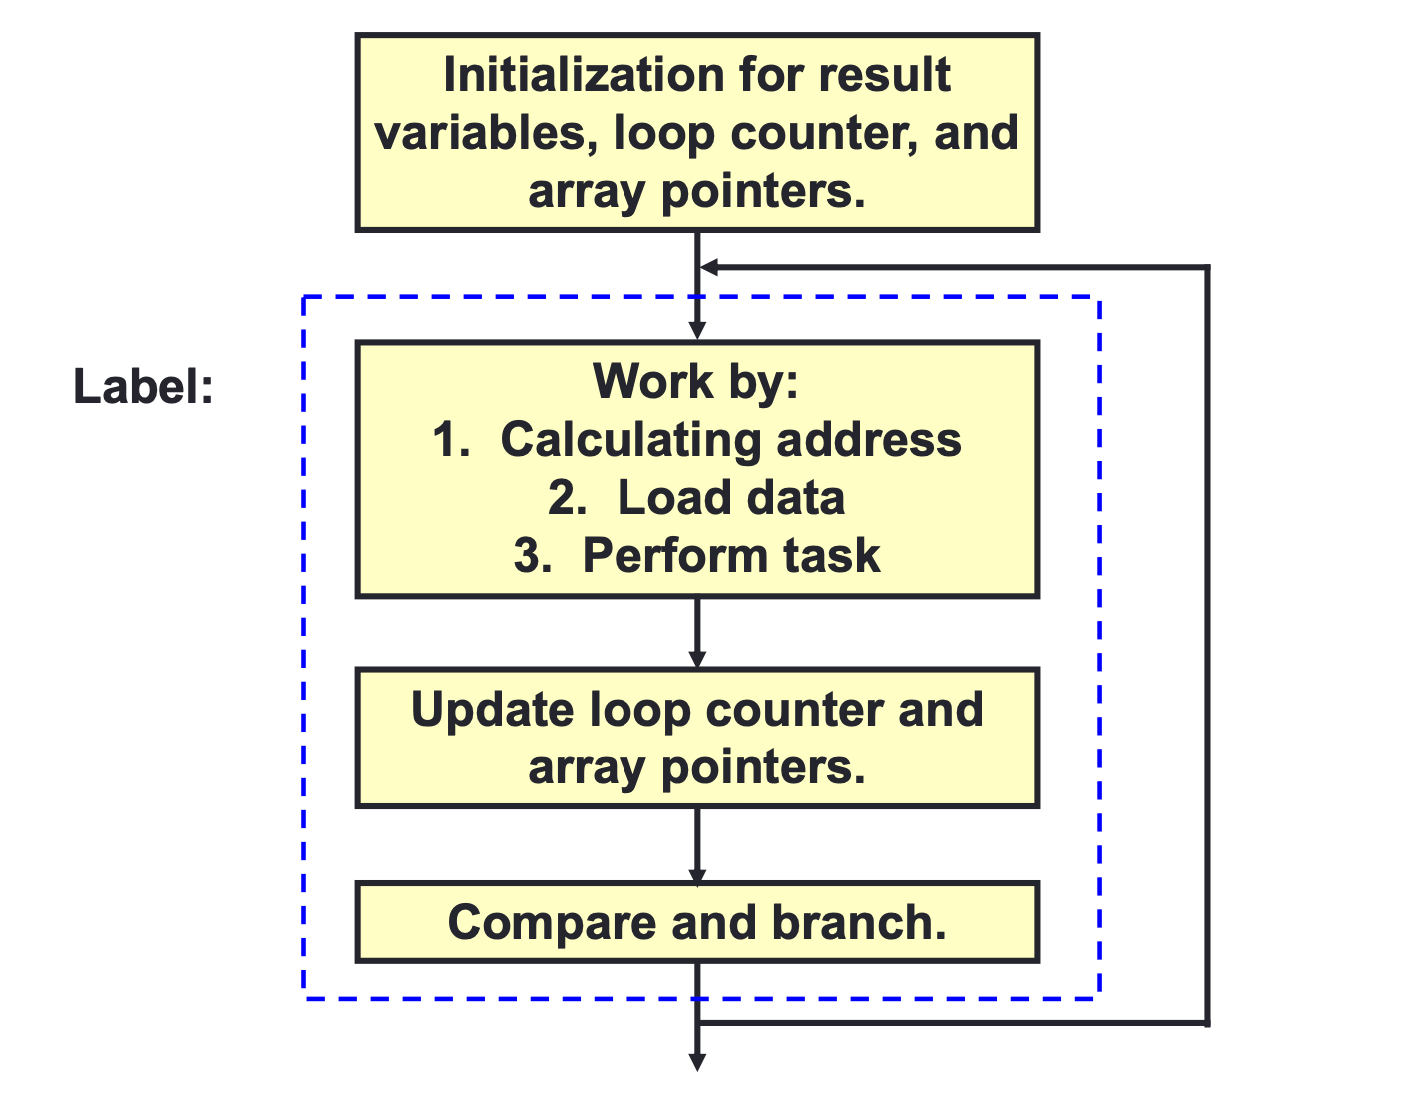
\includegraphics[scale=0.3]{./assets/arrayFlowchart}\\
		Can use pointers instead of index to make code shorter. \\
		- index need to increment, shift left twice (if 4 bytes like int) unless array of chars, then add to base address\\
		- using pointers, set pointer to base address, increment by 4 each time (if int/ float etc), or increment by 1 if char array\\
		
		\textbf{Encoding Instructions}\\
		Constraints are to encode all instructions in 32 bits, and make them as regular as possible\\
		1. R-format (Register format: \texttt{op \$r1, \$r2, \$r3})\\
		2. I-format (Immediate format: \texttt{op \$r1, \$r2, Immd})\\
		3. J-format (Jump format: \texttt{op Immd})\\
		
		\textbf{R-format}\\
		1. Opcode: 6 bits, 0 for all R-format instructions\\
		2. rs (source register): 5 bits\\
		3. rt (target register, second source register for R-type): 5 bits\\
		4. rd (destination register): 5 bits\\		
		5. shamt (shift amount): 5-bits\\
		6. funct: 6-bits\\
		
		\textbf{I-format}\\
		1. opcode (specifies instruction): 6-bits\\
		2. rs (source register): 5-bits\\
		3. rt (target register): 5-bits\\
		4. immd: 16 bits (16 bits 2s comp signed integer)\\
		
		\textbf{Instruction Address}\\
		- Instructions stored in memory\\
		- Instrcutions are 32-bits long\\
		- Instructionsare word-aligned\\
		Program Counter (PC) is a special register that keeps the address of the instruction being executed by processor\\
		
		\textbf{Branch Instruction Encoding}\\
		Immediate is only 16-bits, addresses are 32 bits. Immediate is not long enough to specify target address\\
		But branches usually only jump small amounts, ie changes PC by small amount\\
		- Specify target address \textbf{relative to PC}\\
		- Since instructions are word aligned, can treat the immediate as number of \textit{words} away from PC\\
		- Can branch up to $2^{15}$ words away from PC, $2^{17}$ bytes\\
		Branch Calculation:\\
		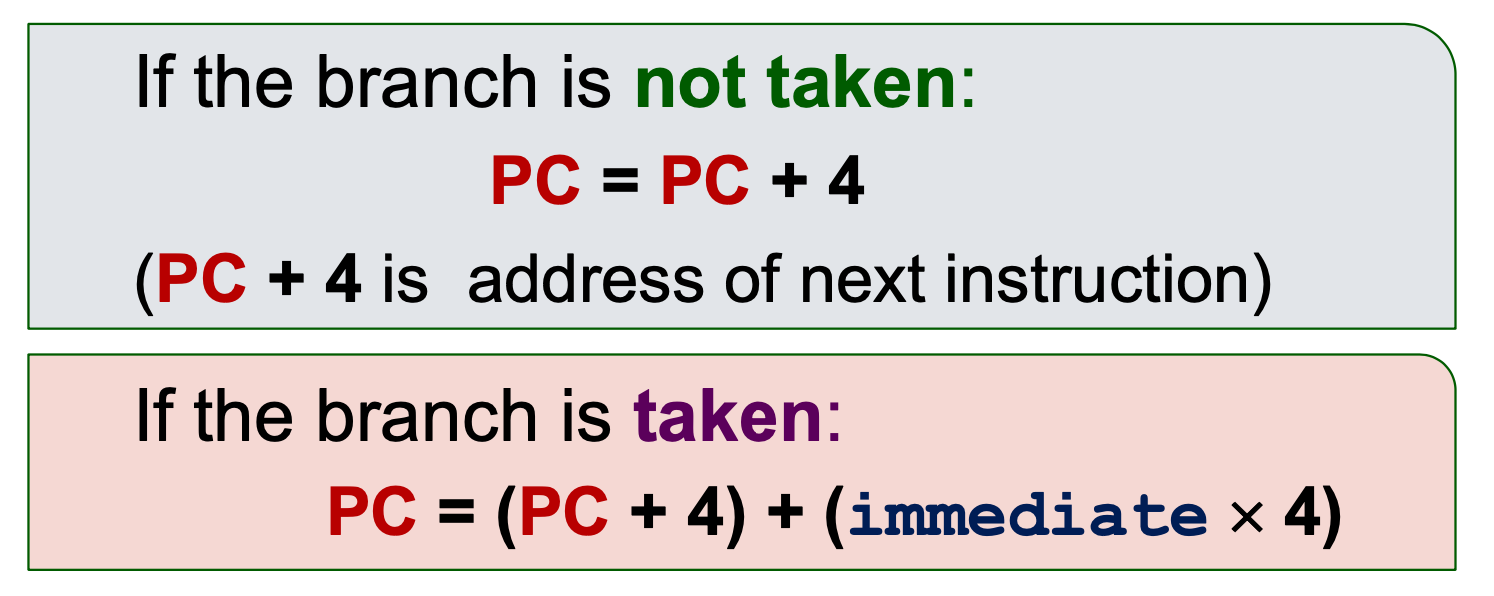
\includegraphics[scale=.25]{./assets/branchCalculation}\\
		Note: immd field specifies number of words to jumps, which is the \textbf{same} as the number of instructions to skip over\\
		Note: add immd to PC + 4 not PC due to hardware design\\
		
		\textbf{J-format}\\
		For jumps, can jump anywhere in memory, not small jumps so cannot use PC-relative addressing\\
		Want to specify a 32-bit address to jump to, but cannot due to 6-bit opcode\\
		Getting the address:\\
		1. Start with 26-bits\\
		2. Instructions are word aligned, so last two bits are always 00, can omit (like branching), now have 28-bit\\
		3. Choose \textbf{4 most significant bits from PC+4}, cannot jump to anywhere in memory but should be sufficient. Max jump range: 256MB boundary\\
		
		\textbf{Summary}\\
		- Branches and load/store are both I-format instructions, but branch use \textbf{PC-relative addressing} while load/store uses \textbf{base addressing}\\
		- Jumps use \textbf{pseudo-direct addressing}\\
		- shifts use R-format, but other immediate instructions use I-format\\
		
		{\normalsize\textbf{Instruction Set Architecture}}\\	
		\textbf{5 concepts of ISA design}\\
		1. Data Storage\\
		2. Memory Addressing Modes\\
		3. Operations in Instruction Set\\
		4. Instruction Formats\\
		5. Encoding the Instruction Set\\
		
		\textbf{1. Data Storage}\\
		Concerns are\\
		- Where to store the operands to that the computation can be performed?\\
		- Where to store the result?\\
		- How to specify the operands?\\
		
		Common Storage Architectures\\
		- Stack: Operands are implicitly on top of the stack\\
		- Accumulator: One operand implicitly in the accumulator (special register)\\
		- General Purpose Architecture: Only explicit operands. Register-Memory (one operand in memory) and Register-Register (load-store like MIPS)\\
		- Memory-Memory: all operands in memory\\
		\includegraphics[scale=.25]{./assets/dataStorage}\\
		
		\textbf{2. Memory Addressing Mode}\\
		- Given $k$ bit address, address space is of size $2^k$\\
		- Each memory transfer consists of one word of $n$ bits\\
		Procesor contains:\\
		- Memory Address Register (MAR): k-bit address bus between processor and memory (one direction cpu $\rightarrow$ mem)\\
		- Memory Data Register (MDR): n-bit data bus (bidirectional for read and write)\\
		- control lines: eg read/write control\\
		
		\textbf{Endianness}\\
		The relative ordering of the bytes in a multiple-byte word stored in memory\\
		- Big-endian: MSB stored in lowest address\\
		- Little-endian: LSB stored in lowest address\\
		Eg. For \texttt{0xDE AD BE EF}\\
		- Big-endian: \texttt{0: DE, 1: AD, 2: BE, 3: EF}\\
		- Little-endiand: \texttt{0: EF, 1: BE, 2: AD, 3: DE}\\
		NOTE: Ordering \textbf{within} bytes are not affected, only ordering \textbf{between} bytes\\
		
		\textbf{Addressing Modes}\\
		In MIPS, 3 addressing modes\\
		1. Register: Operands in register\\
		2. Immediate: Operand is specified in instruction directly\\
		3. Displacement: Operand is in memory with address calculated as Base + Offset (lw/sw)\\
		
		\textbf{4. Instruction Format}\\
		Instruction Length:\\
		- Variable length: More flexible (but complex) and compact instruction set, requires multi-step fetch and decode\\
		- Fixed length: Easier fetch and decode, simplify pipelining and parallelism, but instruction bits are scarce\\
		
		\textbf{5. Encoding the Instruction Set}\\
		Things to be decided:\\
		- No. of registers\\
		- No. of addressing modes\\
		- No. of operands in instruction\\
		Expanding Opcode scheme for fixed length instructions\\
		- Opcode has variable length for different instructions\\
		Eg. 16 bit fixed length instruction, 2 types of instructions, 1 operand and 2 operand, each operand takes 5 bits\\
		- Type A: 6-bit opcode, $2 *$5-bit operand\\
		- Type B: 11-bit opcode, $1*$5-bit operand\\
		To maximise no. of instructions: Give more 6-bit prefixes to type B\\
		To minimise no. of instructions: Give more opcodes to type A\\
		
		{\normalsize\textbf{Datapath}}\\
		Components that process data and performs arithmetic, logical and memory operations\\
		
		\textbf{Instruction Execution Cycle}\\
		1. Instruction Fetch: Get instruction from mem (address is in PC)\\
		2. Instruction Decode and Fetch Operands: Find out operation, get operands\\
		3. ALU: Arithmetic and Logical operations\\
		4. Memory Access: Memory operation (load/store)\\
		5. Result Write: Write back result of operation to register if needed\\
		NOTE: can merge instruction decode and operand fetch because decode is simple for MIPS\\
		
		\textbf{1. Instruction Fetch}\\
		1. Use PC to fetch instruction from memory\\
		2. Increment PC by 4 to get address of next instruction (recall instructions are 32-bits long)\\
		Exception is when branch or jump\\
		- Sequential circuit (circuit that can store info?)\\
		- PC is read during first half of the clock period and is updated with PC+4 ad the \textbf{next rising clock edge}, this prevents reading and updating PC at the same time\\
		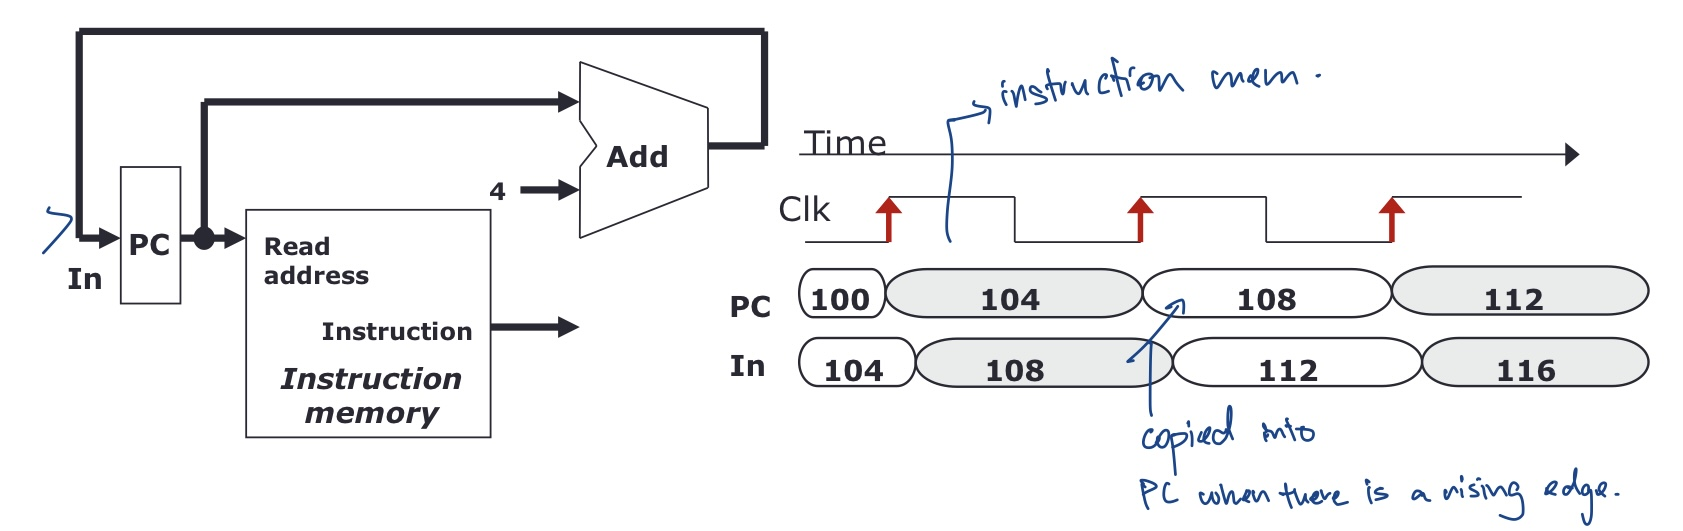
\includegraphics[scale=.15]{./assets/clock}\\
		
		\textbf{2. Instruction Decode}\\
		1. Read opcode to determine instruction type and field lengths\\
		2. read data from necessary registers\\
		- Register File: collection of 32 32-bit registers that can be read or written to\\
		- Each instruction reads at most 2 registers and writes to at most 1 register\\
		- \texttt{RegWrite} is the control signal to indicate writing fo register; 1 = write, 0 = no write\\
		- Need to use multiplexer with \texttt{RegDst} control signal to choose between \texttt{rt} and \texttt{immediate} for write register\\
		- Need to sign extend \texttt{immediate} to 32 bit and output to ALU\\
		Refer to slides\\
		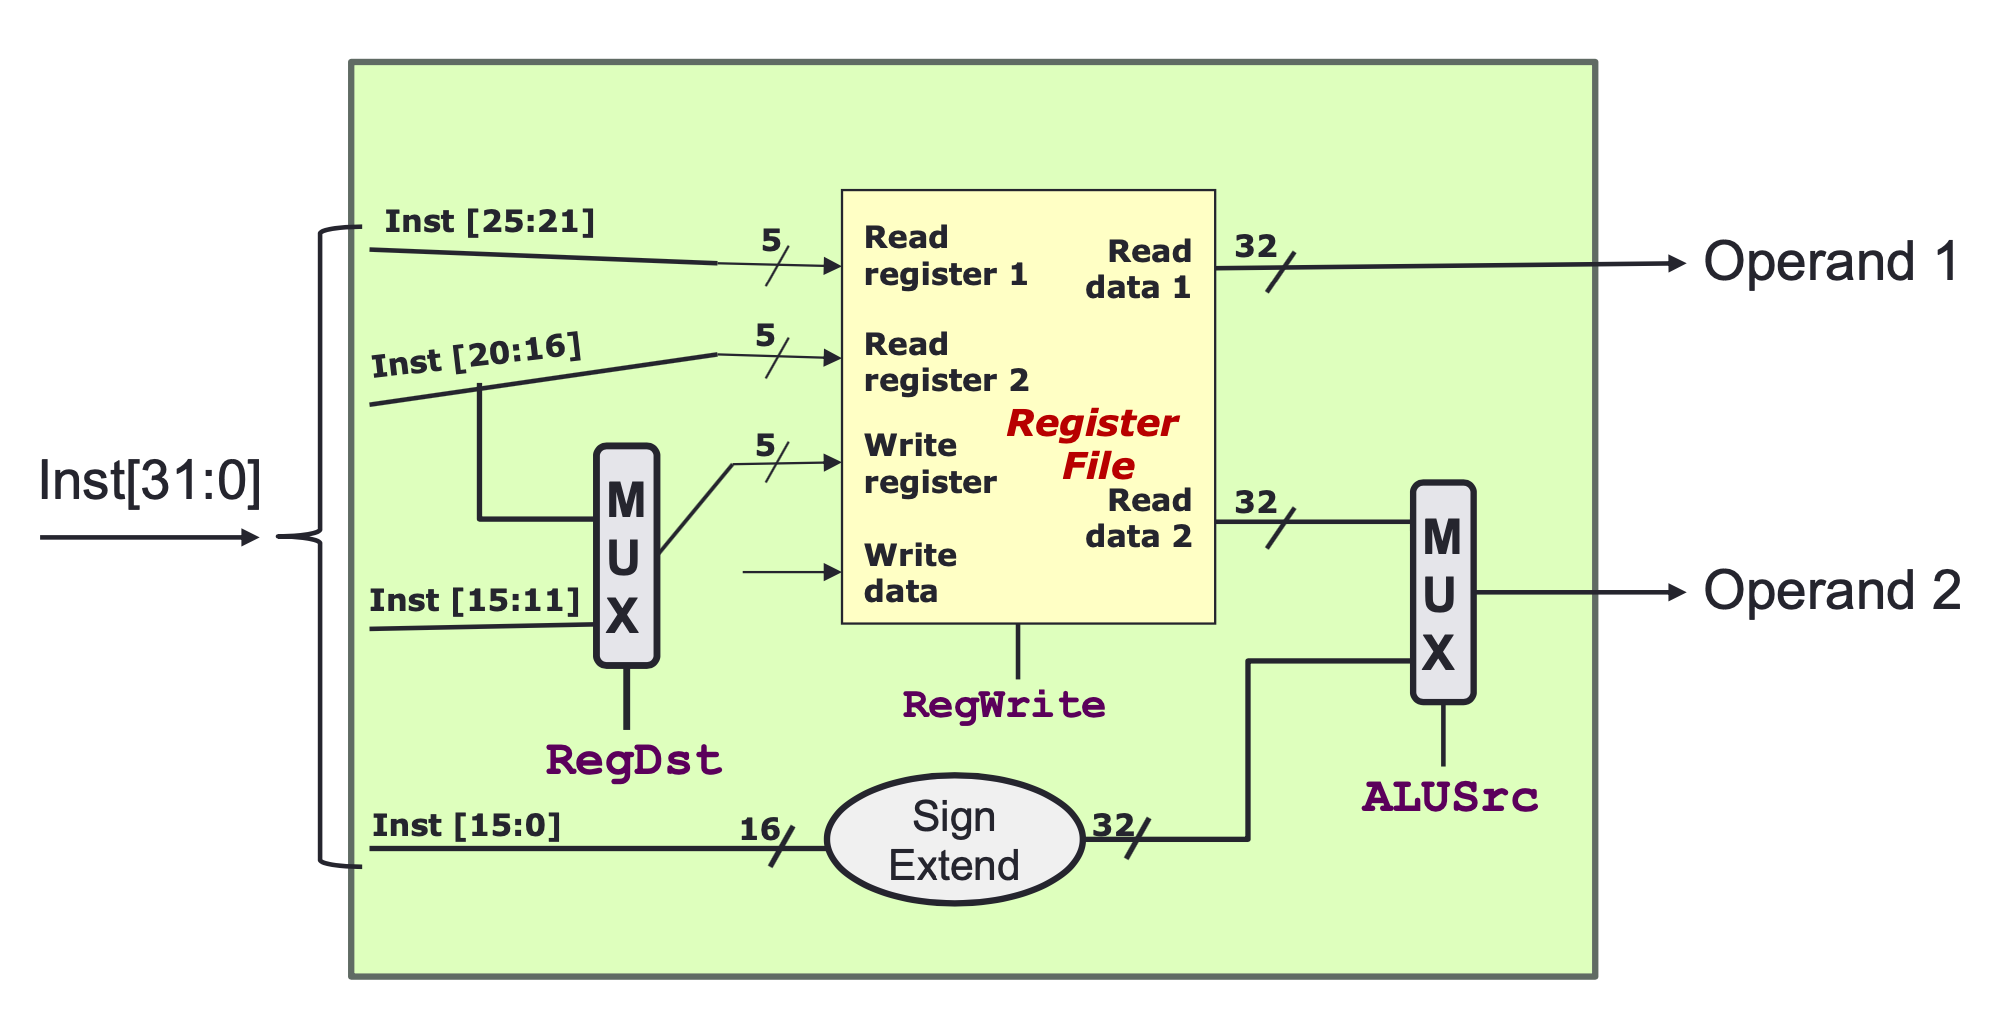
\includegraphics[scale=.27]{./assets/decodeStage}\\
		
		\textbf{3. ALU Stage aka EX stage}\\
		- Performs arithmetic, logical and shifting operations\\
		- Performs register comparison and target address calculation for branching and memory operations\\
		ALU\\
		- Combinational logic to implement operations\\
		- takes in 2 32 bit numbers\\
		- outputs 32-bit result and 1 bit signal \texttt{isZero} for branching\\
		- 4-bit control signal called \texttt{ALUcontrol}\\
		
		Exception Branch instructions\\
		- need to perform 2 calculations: Branch outcome and target address\\
		- current circuit would be wrong because branching is I-format instruction (ALUSrc would send immediate to ALU instead of register)\\
		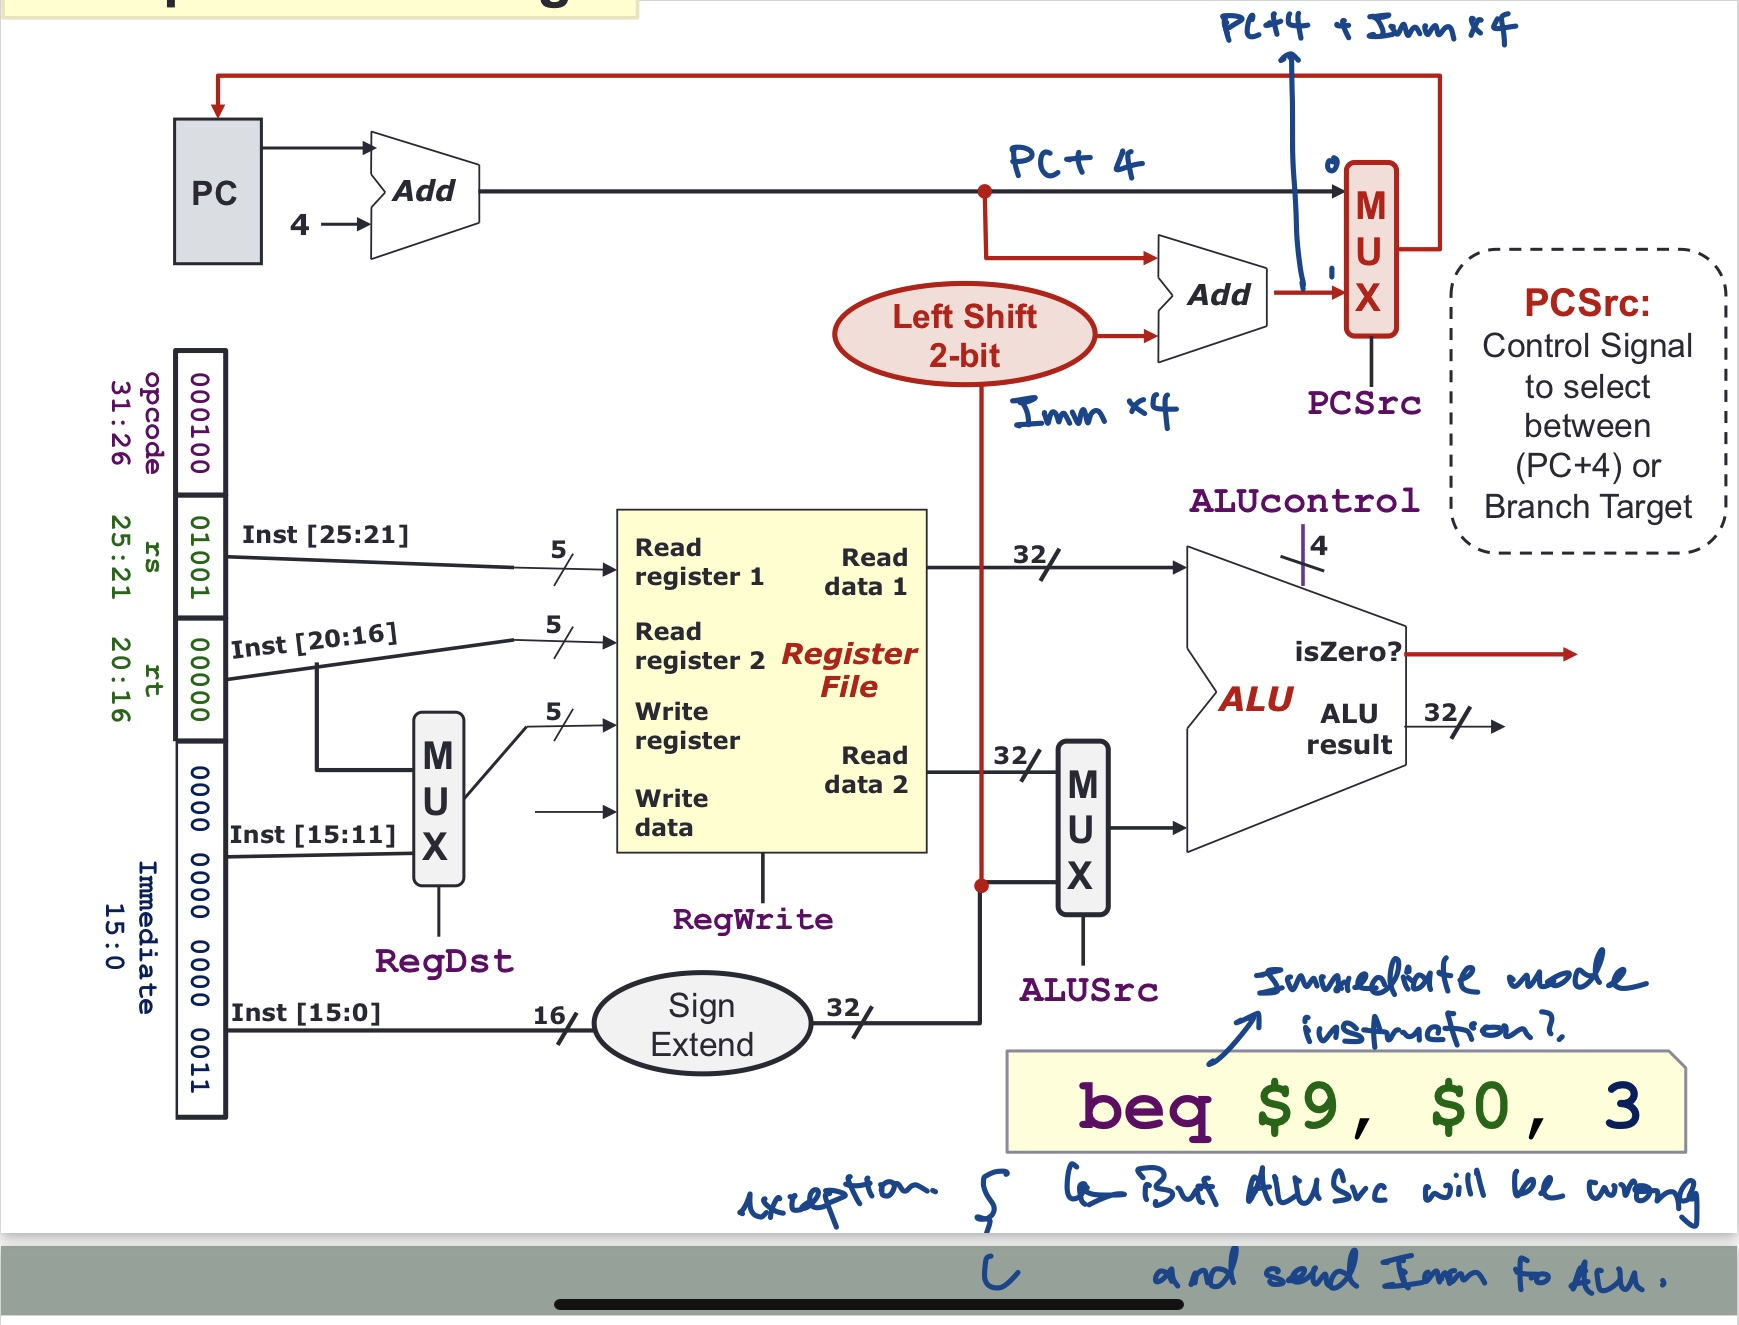
\includegraphics[scale=.15]{./assets/ALU}\\
		
		\textbf{4. Memory Stage}\\
		Only load and store instructions need to perform operations in this stage.\\
		- Use memory address calculated by ALU stage\\
		- Read or write to data memory\\
		All other instructions remain idle\\
		Data memory\\
		- Inputs: memory address, data to be written (Write Data) for store instructions\\
		- Output: Data read from memory for load instructions\\
		- Control: Read and write controls
		\begin{verbatim}
			R W
			1 1 undefined (should not have this case)
			0 1 write
			1 0 read
			0 0 nothing
		\end{verbatim} 
		For store instructions, need to connect RD2 (rt) to Write Data.\\
		Need to choose between output from Read Data and output from ALU stage\\
		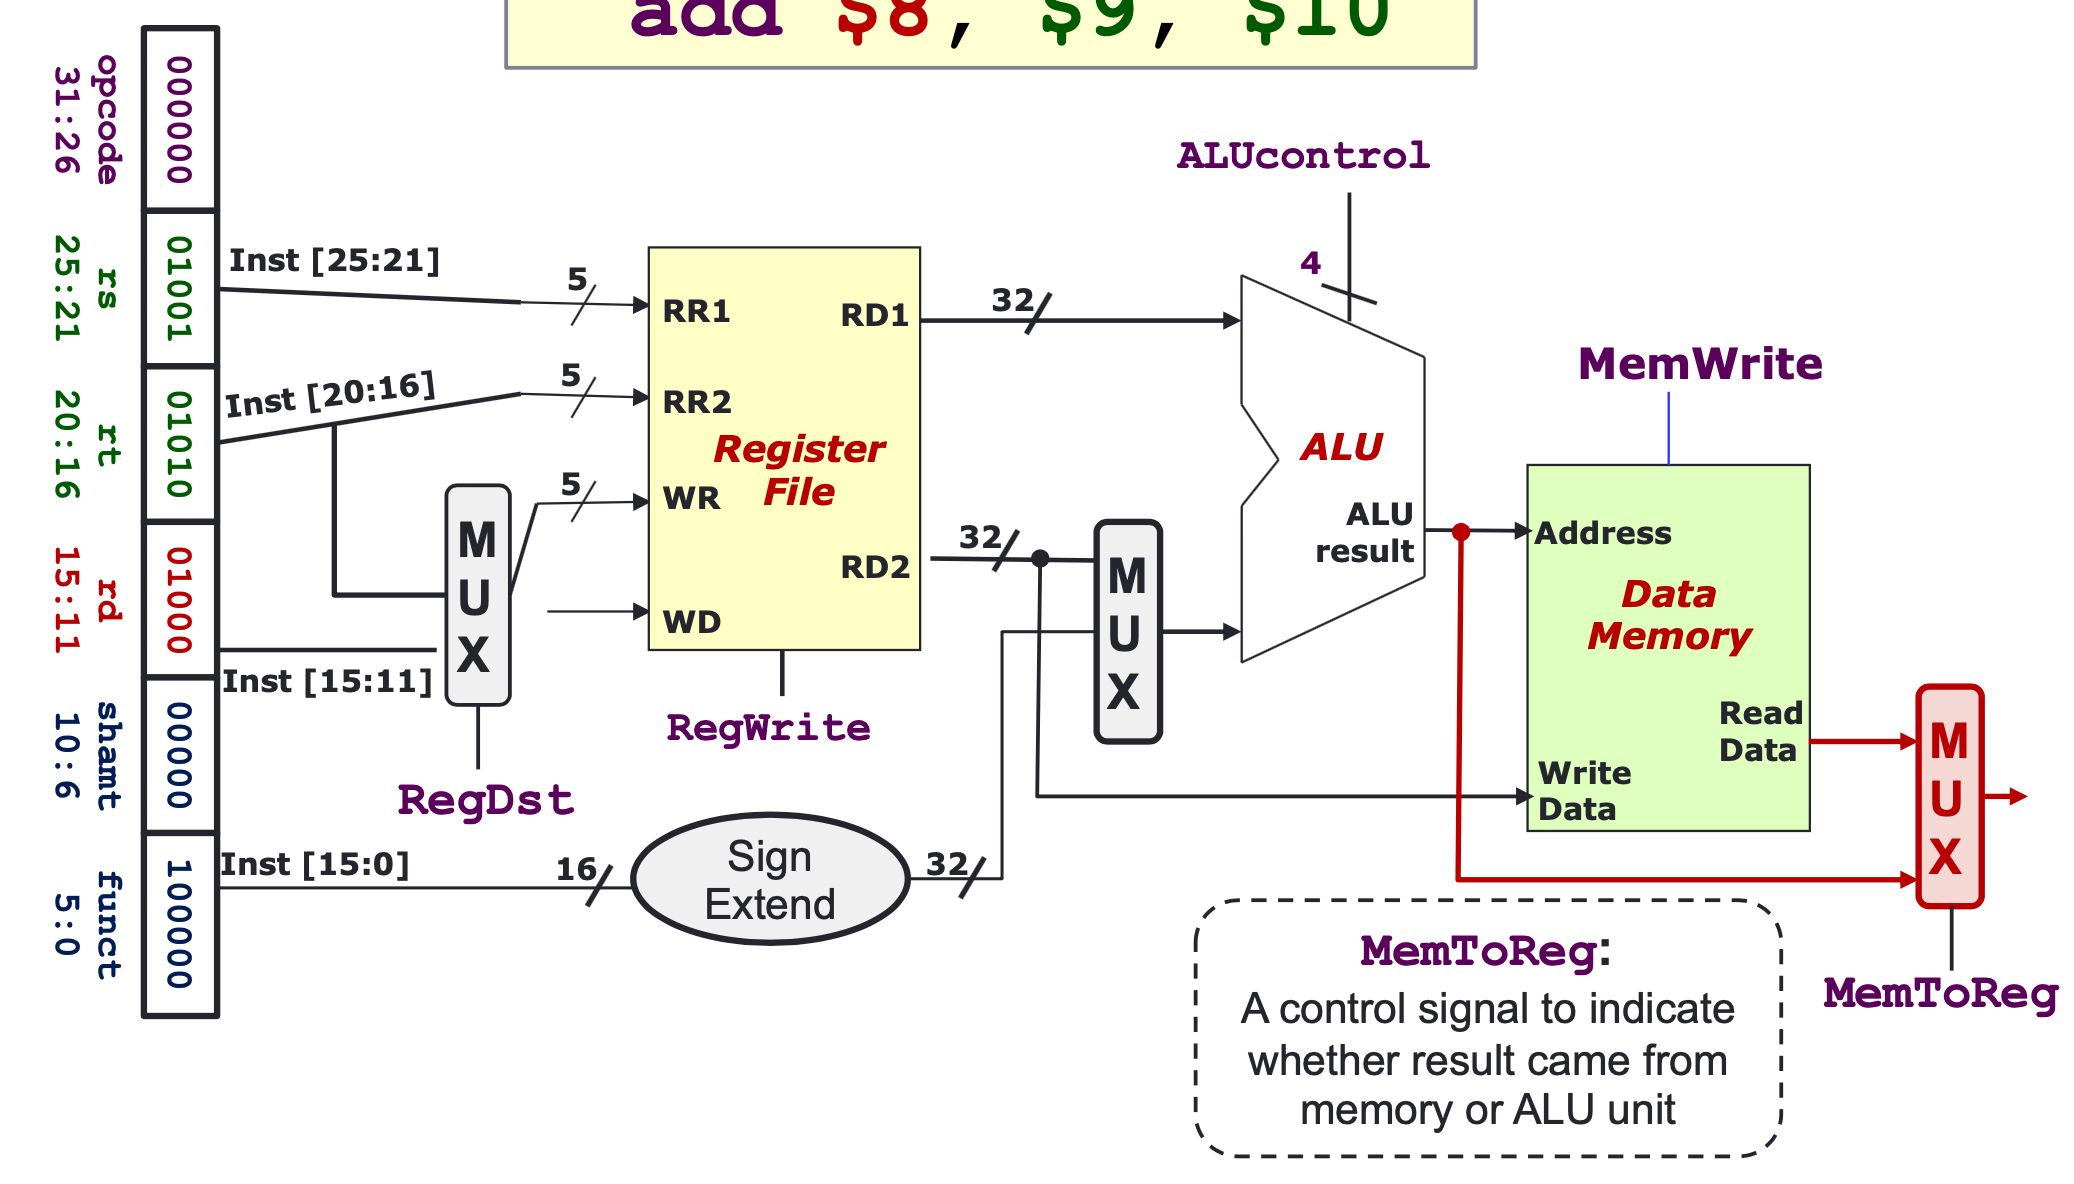
\includegraphics[scale=.25]{./assets/memStage}\\
		NOTE: MemToReg mux is mounted upside down ie. 1 is Read Data, 0 is ALU result\\
		 
		\textbf{5. Register Write Stage}\\
		Write to register (stores, arithmetics, loads, slt, etc)\\
		Just connect correct result to Register File Write Data input.\\
		- Control: RegWrite, 1 write 0 nothing\\
		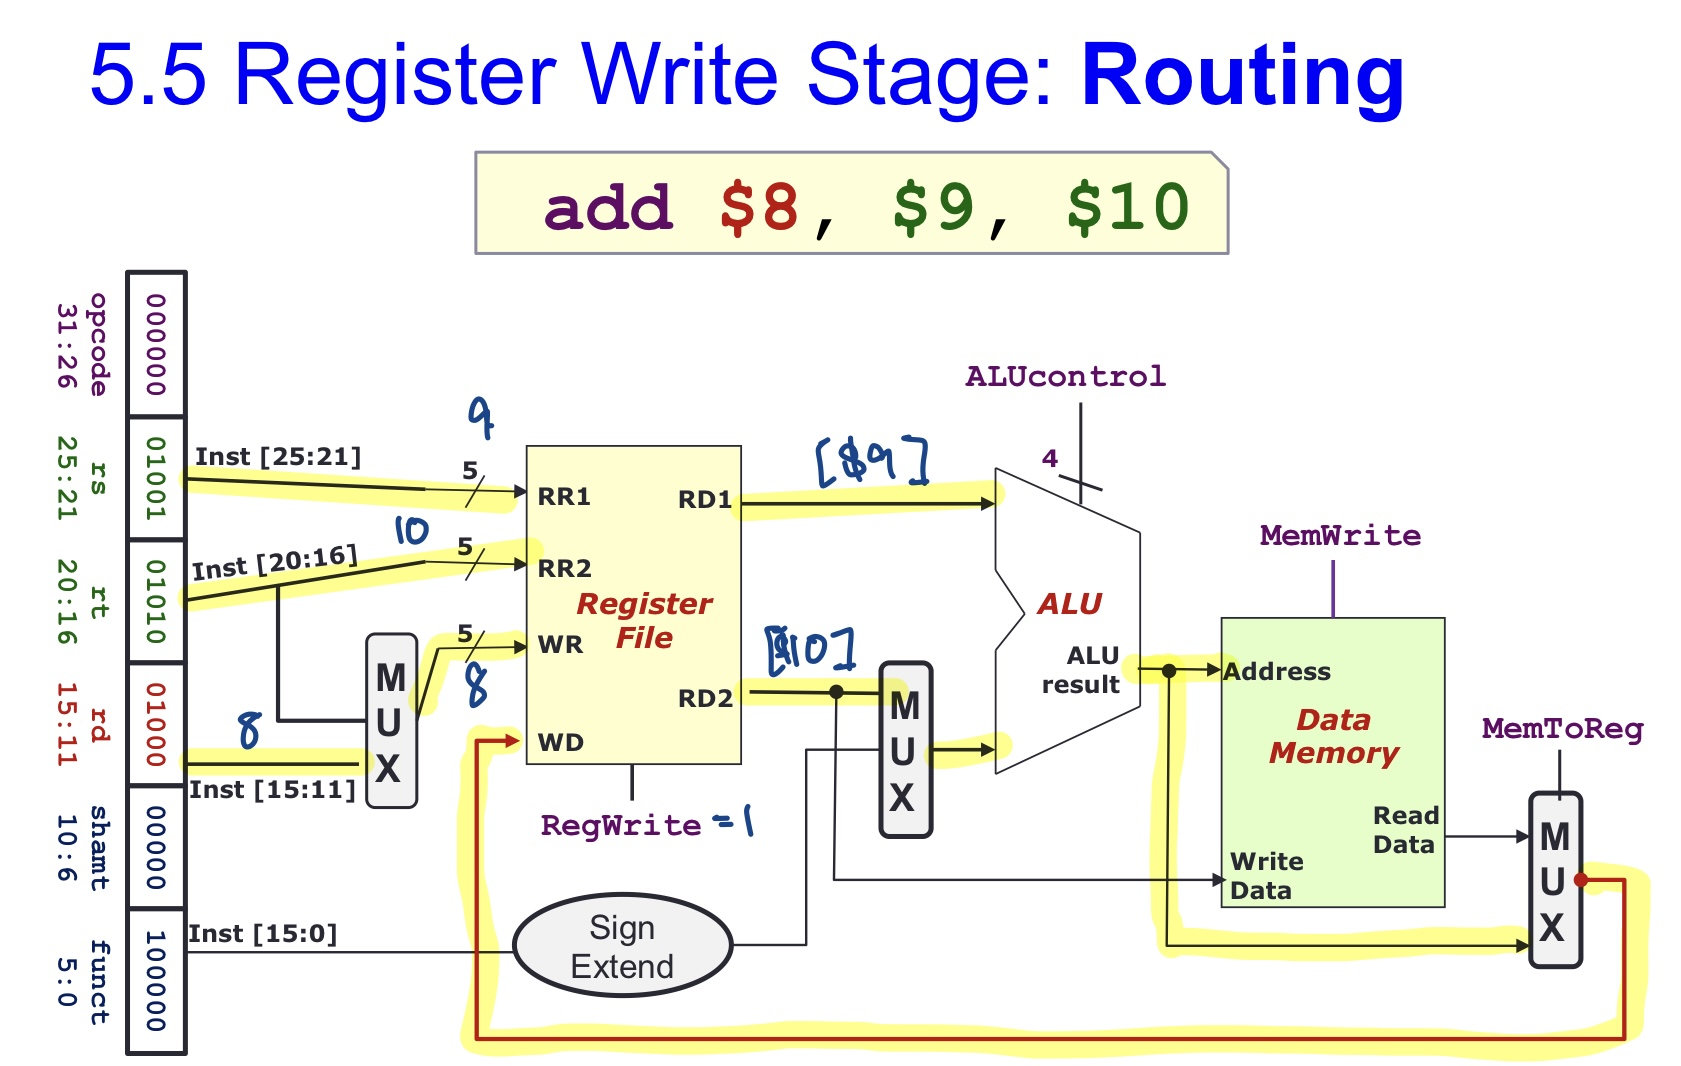
\includegraphics[scale=0.16]{./assets/regWrite}\\
		
		{\normalsize\textbf{Control}}\\
		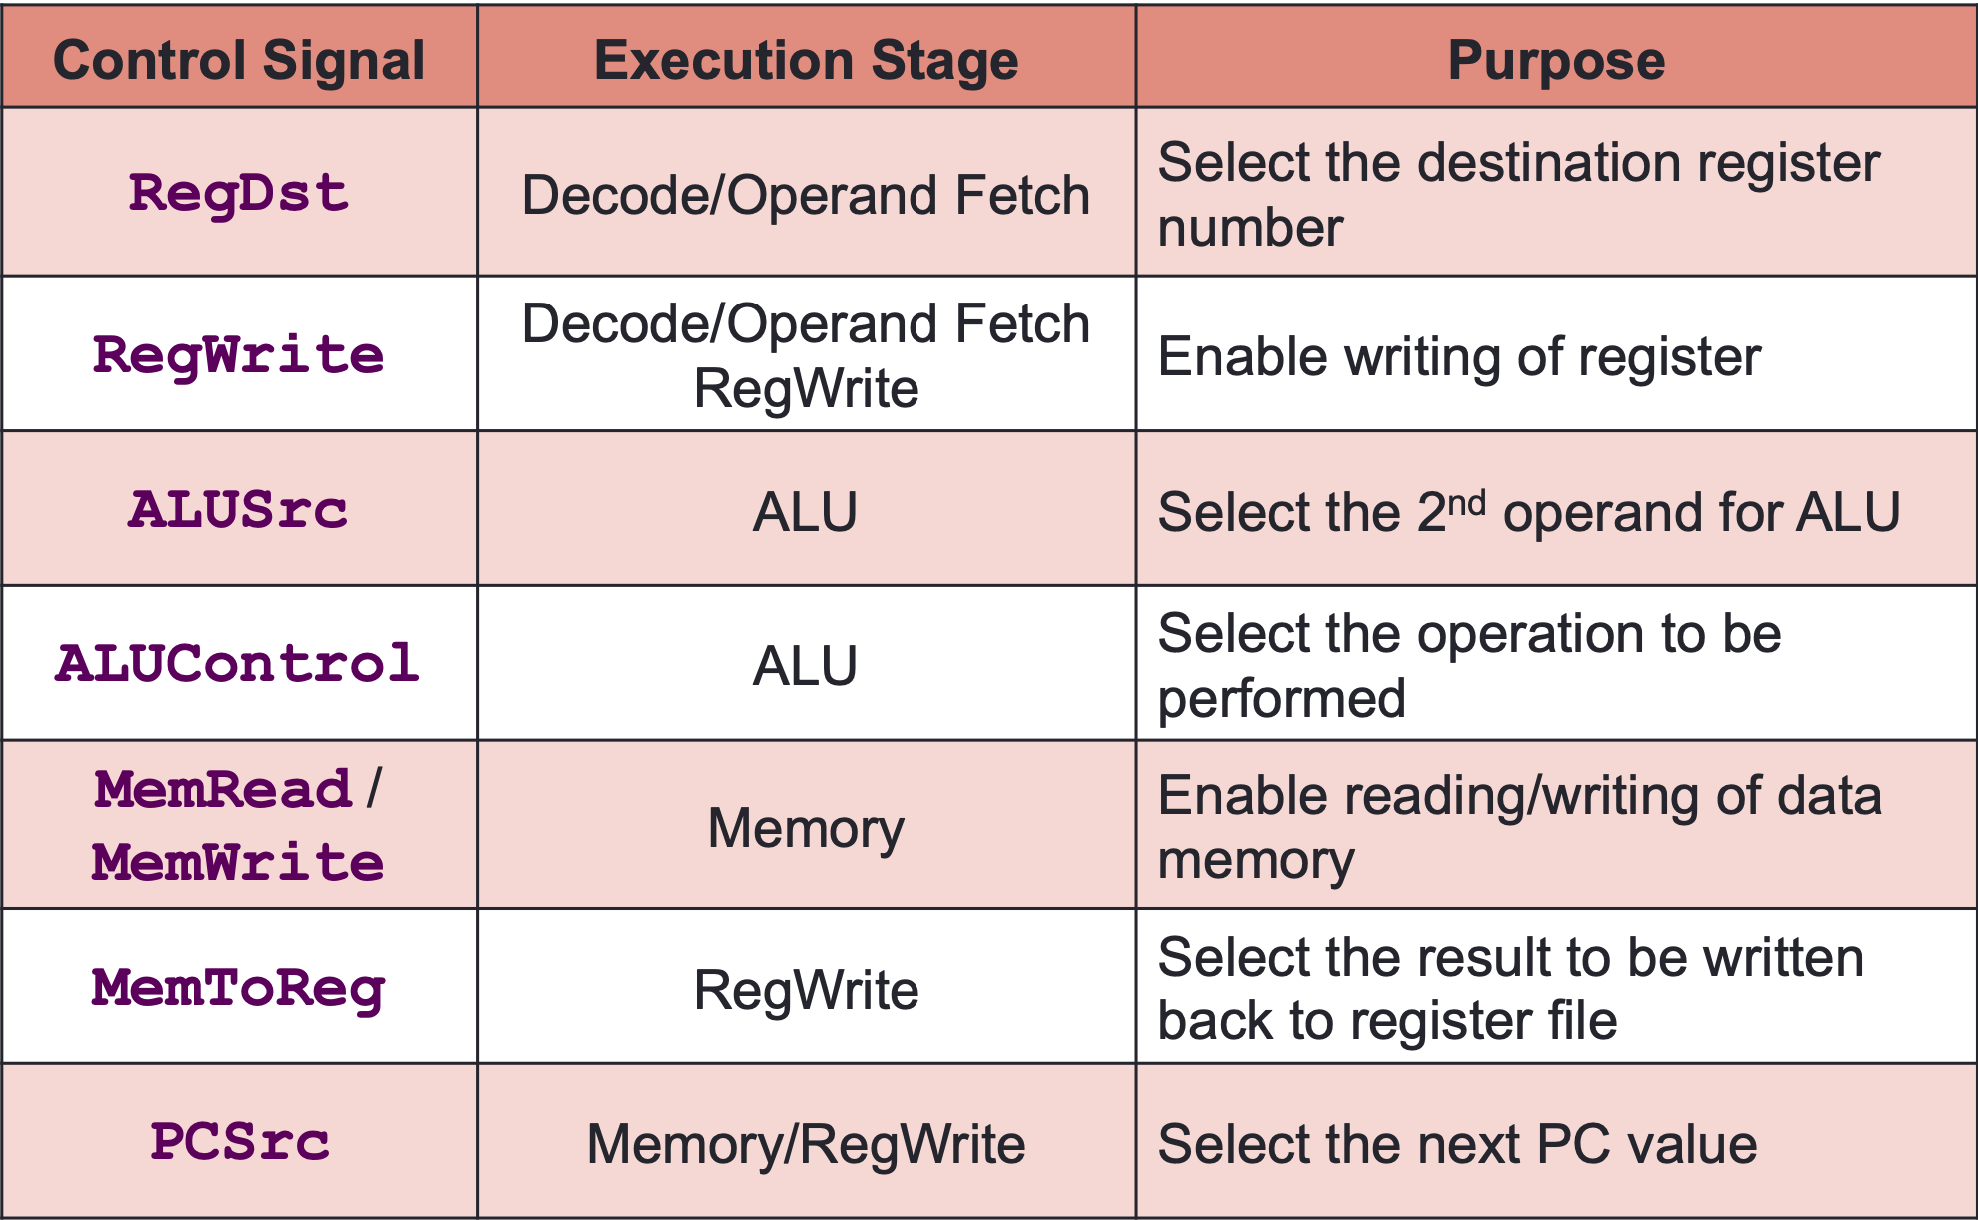
\includegraphics[scale=.26]{./assets/controlSignals}\\
		- Generate all of these signals using opcode (and funct, for R-type) using a combinational circuit\\
		
		\textbf{PCSrc}\\
		Note only need opcode (that it is a branch instruction) but also if the branch is taken (\texttt{isZero === 1}).\\
		- Therefore, need to combine the two signals using \texttt{AND} gate\\
		
		\textbf{ALUControl}\\
		All control signals other than ALUControl can be generated from opcode only (the signals are the same for all R-type), only ALUControl needs funct code (as opcode is 0 for all R-type)\\
		- only exception is shifts?\\
		
				
				
				
		
		
		
		
		
		
				
	\end{multicols*}

\end{document}
